\listfiles
%rfr 在tex文件顶部使用"\listfiles"命令,编译后生成的log文件将包含使用的宏包列表(及其版本号),可以参考:https://mp.weixin.qq.com/s/Xkfaxo_EPTGxam5DL_veOQ

\documentclass{ctexart} 

% 封面
\title{简单高效\LaTeX( 吴康隆)学习笔记\thanks{This is a footnote in the title.}}
\author{殷元昊\thanks{This is a footnote in the author.}}
\date{}
            % "\title{title}和"\author{}"是必须定义的,"\date{text}"如果省略,会自动以编译当天的日期为准,如果不想显示日期,可以输入"\date{}"
            % 标题页的脚注用"\thanks{text}"命令完成

% 宏包-----------------------------------------------------------------------------------------------------------------------------------

% \usepackage{ctex}

\usepackage{lipsum}
            %rfr lipsum宏包提供"\lipsum"命令,用于生成一段无意义的测试文本,默认输出150段中的前7段,可以通过可选参数来指定输出的段落序数,比如:"\lipsum[4-57]"(第4段到第57段)、"\lipsum[23]"(第23段),还可以通过第二个可选参数指定输出段落中的句子序数,比如:"\lipsum[3-9][4-8]"(第3段到第9段当中,每一段的第4句到第8句),可以参看其官方手册:https://jp.mirrors.cicku.me/ctan/macros/latex/contrib/lipsum/lipsum.pdf
            %* 经检验,无法在一个指定参数中指定不连续的段落或者句子,比如"\lipsum[2,4]"、"\lipsum[2-4][1,3]"都无法输出正确的结果

\usepackage{blindtext}
            %rfr blindtext宏包提供"\blindtext"命令,生成一段无意义的测试文本,可以通过可选参数来指定重复次数(重复后的多段文本在一个段落内首尾相接);"\Blindtext"命令用于生成五段相同的上述文本,可以通过可选参数来控制重复的段落数,默认值为5,可以通过第二个可选参数来控制每个段落内文本的重复次数(相当于"\blindtext"命令的可选参数);"\blinddocument"命令用于生成一篇带有章节名(section、subsection……)、列表(itemize、enumerate、description)等内容的文档;"\Blinddocument"命令用于生成一篇更长的类似文档,可以参考其官方手册:https://jp.mirrors.cicku.me/ctan/macros/latex/contrib/blindtext/blindtext.pdf

\usepackage[normalem]{ulem}
            % ulem宏包,提供各种下划线和删除线,normalem选项可以防止\emph{}命令的效果变成加下划线

\usepackage{hologo}
            % hologo宏包可以输出许多TeX家族标志


\usepackage{lettrine}
            % 宏包lettrine能够生成首字下沉的效果

\usepackage{indentfirst}
            %* article文档类下,即使在首行开头使用"\indent"命令,以英文字母开头的首行也不缩进,解决方法有三种:(1)加载indentfirst宏包,这是最常用的办法;(2)加载ctex宏包;(3)设置文档类为ctexart
            %rfr 第二种和第三种方法设置的首行缩进效果会被下文提到的titlesec宏包的"\titlespacing*{command}{left}{before-sep}{after-sep}"命令消除,由此也可以看出加载indentfirst宏包是防止首行不缩进的最好的办法

% \usepackage{parskip}
            %rfr 强制所有段首不缩进,参考:https://tex.stackexchange.com/questions/196922/indent-first-paragraph-after-section-and-dont-indent-new-lines

\usepackage{fontspec} 
            % 在XelaTeX编译下,使用fontspec宏包来选择本地安装的字体。注意,该宏包可能会明显增加编译时间

\usepackage[slantfont,boldfont]{xeCJK} 
            % "slantfont"和"bolfont"选项表示允许设置中文的斜体和粗体字形

    \setCJKmainfont[boldfont = SimHei]{SimSun} 
            % 设置"SimSun"(宋体)为主要字体,"SimHei"(黑体)为主要字体的粗体字形,即"\textbf{}"或者"{\bfseries}"命令的变换结果。也可以通过slantfont选项来设置主要字体的斜体字行
            %* 各章节的汉字字形也因此发生变化
            %! 注意,"SimSun"和"SimHei"名称中的大小写一定要写对,否则编译会报错

\usepackage{pifont} 
            %* 用于输出图标(symbol fonts)的宏包

\usepackage{xcolor} 
            % 使用xcolor宏包来方便地调用颜色
            % 提供"\colorbox{color}{text}"、"\fcolorbox{color}{color}{text}"命令

\usepackage{amsmath} 
            % 宏包amsmath提供了"\eqref"命令,输出默认形式如"(3.1)"所示的数值

% \usepackage{nameref} 
            % nameref宏包不满足于只引用编号,还提供了引用对象的标题内容的功能

\usepackage{lastpage} 
            % lastpage宏包提供的标签"LastPage"可以保证打印出整个文档最后一页的页数

\usepackage[perpage,bottom]{footmisc} 
            % footmisc宏包的perpage选项可以让脚注每页重新编号,默认情况下,脚注按章编号
            %* bottom的可选参数可以使得脚注始终处于默认页面区域的底部,而不会因为LaTeX的提前分页操作导致上移到实际页面区域的底部

\usepackage{endnotes} 
            % 用于设置尾注的宏包

\usepackage{csquotes} 
            %* 管理在正文中引用文本的宏包

\usepackage[numbers,sort&compress,super,square]{natbib} 
            % 使用natbib宏包可以定制参考文献标号在文中的显示方式
% \usepackage{natbib} 
            %* 只加载natbib宏包,编译会报错
% \usepackage[numbers]{natbib} 
            % 数字编号
            %* 单独设置该选项,编译成功
% \usepackage[sort&compresss]{natbib} 
            % 排序且压缩
            %! 单独设置该选项,编译会报错
% \usepackage[super]{natbib} 
            % 上标
            %* 单独设置该选项,编译成功
% \usepackage[square]{natbib} 
            % 外侧方括号
            %! 单独设置该选项,编译会报错

\usepackage[numbib,numindex]{tocbibind}
            %* "toc"是"table of contents"的缩写  
            %* 使用tocbibind宏包将目录本身、图目录、表目录、索引、参考文献全部编入目录,并且给参考文献章节和索引章节正常编号
            %* 但是并没有专门为图目录和表目录的正常编号设置的可选参数  
% \usepackage[nottoc]{tocbibind} 
            % 目录本身不编入目录
% \usepackage[notlof]{tocbibind} 
            % 图目录不编入目录
% \usepackage[notlot]{tocbibind} 
            % 表目录不编入目录
% \usepackage[notindex]{tocbibind} 
            % 索引不编入目录
% \usepackage[notbib]{tocbibind} 
            % 参考文献不编入目录
% \usepackage[numindex]{tocbibind} 
            % 给索引章节正常编号
% \usepackage[numbib]{tocbibind} 
            % 给参考文献章节正常编号
% \usepackage[none]]{tocbibind} 
            % 禁用所有

\usepackage[section]{placeins}
            % 重新定义了"\section{}"命令,在此之前加上了"\Float-Barrrier"命令,阻止浮动体跨过该位置

\usepackage{graphicx}
            % 使用graphicx宏包和"\includegraphics[options]{name}"命令插入图片
            % 提供"\scalebox{h-scale}[v-scale]{text}"和"\rotatebox[keyvals]{angle}{text}"命令

\usepackage{caption}
            % caption宏包用来设置浮动体的标题格式

\usepackage{subcaption}
            %* 使用subcaption宏包提供的subfigure环境,在figure环境中嵌套多图
            % 使用subcaption宏包提供的subtable环境,在table环境中嵌套多张表格
            %! 注意,subcaption宏包和subfig宏包只能加载其中一个,否则编译会报错

% \usepackage{subfig}
            % 使用subfig宏包提供的"\subfloat[sub-caption]{body}"命令,在figure环境中嵌套多图
            %! 注意,subcaption宏包和subfig宏包只能加载其中一个,否则编译会报错 
            
\usepackage{wrapfig}
            % 使用wrapfig宏包进行图文混排

\usepackage{multirow}
            % 使用multirow宏包解决跨行跨列的问题

\usepackage{array} 
            % array宏包提供"m{}"、"b{}"、">{decl}"、"<{decl}"、"!{intercolumn sign}"、"\newcolumntype{name}{definition}"等命令

\usepackage{tabularray} 
            %* tabularray宏包提供使文本靠近表格上端或者下端的命令

\usepackage{makecell} 
            % makecell宏包提供了一种方便在单元格内换行的方式,以及设置水平表线宽度的命令

\usepackage{diagbox} 
            % diagbox宏包提供了分割表头的命令

\usepackage{tabularx} 
            % tabularx宏包的tabularx环境使得表格可以通过在每列上均匀增加列宽的方式设置整表宽度

\usepackage{dcolumn} 
            % dcolumn宏包提供了小数点对齐的对齐方式

\usepackage[showframe]{geometry}
    % \geometry{twoside}
            % 借助geometry宏包进行页面设置
            %* twoside选项会影响到边注命令"\marginpar[left]{right}"中可选参数对应的内容在偶数页上的显示位置,如果不设置twoside选项,则偶数页上的边注都一律显示在右侧,参见"3.5.2 脚注、边注与尾注"一节

\usepackage{fancyhdr}
            % 借助fancyhdr宏包控制页眉和页脚
            %* "hdr"应该是来自"header"的缩写
    \pagenumbering{arabic}
            % 设置页码的格式,默认值为arabic,还可以设置为Roman、roman、Alpha、alpha
    \pagestyle{fancy}
            % 设置页眉和页脚的格式,还可以设置其他值,包括:empty(无页眉、页脚)、plain(无页眉,页脚只包含一个居中的页码)、headings(无页脚,页眉包含章节编码、章节名称与页码)、myheadings(无页脚,页眉包含页码和用户定义的信息,经检验,默认情况下只包含页眉中的页码)
            %* 在单边模式下,如果不使用"\pagestyle{fancy}"命令,每一页都会显示不带下边线的页眉,不显示页脚,正文部分的第一页和第二页只在页眉的右侧显示页码,从第三页开始,在页眉的左侧显示次节(subsection)编号和次节名称,在页眉的右侧显示页码;如果使用"\pagestyle{fancy}"命令,每一页都会显示包含下边线的页眉以及不带基线的页脚,正文部分的第一页和第二页只在页眉的右侧显示节(section)编号和节名称,在页脚处显示页码,从第三页开始,在页眉的左侧显示次节(subsection)编号和次节名称,在页眉的右侧显示节(section)编号和节名称,在页脚处显示页码
            %* 在双边模式下,如果不使用"\pagestyle{fancy}"命令,奇数页显示不带下边线的页眉,偶数页显示页脚,正文部分的第一页只在页眉的右侧显示页码,正文部分的第二页只在页脚处显示页码,从第三页开始,奇数页在页眉的左侧显示次节(subsection)编号和次节名称,在页眉的右侧显示页码,偶数页在页脚处显示页码;如果使用"\pagestyle{fancy}"命令,每一页都显示带下边线的页眉和不带基线的页脚,正文部分的第一页只在页眉的左侧显示节(section)编号和节名称,在页脚处显示页码,正文部分的第二页只在页眉的右侧显示节(section)编号和节名称,从第三页开始,奇数页在页眉的左侧显示节(section)编号和节名称,在页眉的右侧显示次节(subsection)编号和次节名称,在页脚处显示页码,偶数页在页眉的左侧显示次节(subsection)编号和次节名称,在页眉的右侧显示节(section)编号和节名称,在页脚处显示页码
            %rfr 事实上,上述提到的【节(section)编号和节名称】在页眉和页脚的设置中被属于“较高级别”(higher-level)的信息,【次节(subsection)编号和次节名称】属于“较低级别”(lower-level)的信息,这是在article文档类中的情况,在book文档类中,“较高级别”则是章(chapter),“较低级别”则是节(section),关于页眉和页脚的设置原理的详细介绍,可以参考:https://www.overleaf.com/learn/latex/Articles/How_does_LaTeX_typeset_headers_and_footers%3F#Commands_for_the_output_routine
%* 注意,如果同时设置empty/plain/headings/myheadings参数和以下命令,优先适用前者,以下命令都不会生效,只有将"\pagestyle{}"命令设置为"fancy"参数,以下命令才会生效
    % \lhead{} 
    %             % 设置页眉左侧的内容,没有内容表示清空默认情况下的内容
    % \chead{} 
    %             % 设置页眉中间的内容
    % \rhead{} 
    %             % 设置页眉右侧的内容,没有内容表示清空默认情况下的内容
    % \lfoot{} 
    %             % 设置页脚左侧的内容
    % \cfoot{} 
    %             % 设置页脚中间的内容,没有内容表示清空默认情况下的页码
    % \rfoot{} 
    %             % 设置页脚右侧的内容
    \renewcommand{\headrulewidth}{.4pt}
                % 设置页眉下边线的高度(不是宽度),默认值为0.4pt
    \renewcommand{\footrulewidth}{.4pt}
                % 设置页脚基线的高度(不是宽度),默认值为0pt
    % \fancyhf[HOR]{元昊} 
            % 可选参数中可以通过三个字母(大小写均可,前后顺序可以变化)来设置内容位置:H/F代表“页眉/页脚”,E/O代表“偶数页/奇数页”,L/C/R代表“左侧/中间/右侧”
            %* 这一命令相比之前几条设置页眉/页脚的命令,优势在于可以同时设置多个位置的页眉/页脚,并且可以分奇偶页进行设置,也可以单独设置"\fancyhead[places]{header}"或者"\fancyfoot[places]{footer}"
% 也可以通过"\fancypagestyle{style name}{definitions}"命令自定义页眉和页脚格式
    % \fancypagestyle{newstyle}{
    %     \fancyhf{} % 清空页眉和页脚
    %     \fancyhead[c]{\thesection} % 在页眉中间显示节(section)的计数器内容
    %     \fancyfoot{\thepage} % 由于没有指定位置,因此在页脚的左中右三个位置处均显示页码
    %     }
    % \pagestyle{newstyle}

\usepackage{shortvrb}
            % shortvrb宏包支持以一对符号代替"\verb"命令

% \usepackage{cuted}
            %* cuted宏包提供strip环境,用于解决figure*环境中的图片在双栏模式下无法在首页被插入的问题
            %! 注意,在strip环境中需要使用caption宏包提供的"\captionof{float type}{heading}"命令来设置标题

% \usepackage{dblfloatfix}
            %* dblfloatfix宏包用于解决figure*环境中的图片在双栏模式下无法在底部被插入的问题,但是仍然无法解决图片无法在首页被插入的问题
            %! 注意,dblfloatfix宏包和stfloats宏包不兼容,只能加载其中一个
            %* 但是dblfloatfix宏包可以和nidanfloat宏包兼容

% \usepackage{stfloats} 
            %* stfloats宏包可以同时解决上述两个问题

% \usepackage{nidanfloat} 
            %* nidanfloat宏包也可以同时解决上述两个问题
            %! 注意,加载nidanfloat宏包会导致通过cuted宏包提供的strip环境中的图片消失,但编译不会报错

\usepackage{multicol}
            % multicol宏包提供multicols环境,可以使同一页内分栏与单栏并存,或者分成多栏,但是此时将无法使用不带星号的浮动体和边注
            %! 注意不要将multicols环境和表格中用于合并列的"\multicolumn{n}{cols}{text}"混淆

\usepackage{import} 
            %* import宏包提供了"\import{full path}{file}"命令和"\subimport{relative path}{file}"命令,前者类似"\input{}"命令,后者可以嵌套使用:在文件一中使用"\import{full path}{file}"命令引用文件二,在文件二中使用"\subimport{relative path}{file}"命令引用文件三,这样就可以直接在文件一中使用"\import{full path}{file}"命令引用文件三
            %rfr 可以参考import宏包的官方手册:https://ftp.kddilabs.jp/CTAN/macros/latex/contrib/import/import.pdf,其中关于相对路径的说明:"The 〈full-path〉 argument for \import can be a full absolute path or a relative path starting from the main working directory for the document."

\usepackage{boxedminipage}
            % boxedminipage宏包提供加框小页环境
            
\usepackage{changepage}
            % changepage宏包提供了一个adjustwidth环境,能够控制段落两侧到文本区的距离

\usepackage{titlesec}
            % 通过titlesec宏包自定义正文中的章节样式
            %rfr 以下关于titlesec宏包和titletoc宏包的各项命令的具体的参数设置可以参考吴康隆(102-107)以及titlesec/titletoc宏包的官方手册:https://mirror-hk.koddos.net/CTAN/macros/latex/contrib/titlesec/titlesec.pdf
    \titlelabel{\thetitle.\quad}
            % 设置各级章节标签格式,在所有章节标签后面多加一个"."符号,默认值为"\thetitle\quad"
            %* "\thetitle"命令指代的就是各级章节标签(计数器),也可以替换成"\thesection"、"\thesubsection"等,但是最好替换成最低一级的章节计数器,因为章节标签只会打印到所指定的那一级,低于指定等级的章节标签会全部消失。即使这样,也仍然不建议将"\thetitle"命令替换成最低等级的章节计数器,因为这会导致所有章节标签被重新定义,例如本文档中已经将节一级的标签重定义为“第X章”的形式,如果此处将"\thetitle"替换为"\thesubsubsection",将会导致节一级的标签显示为"X.0.0"的形式
    \titleformat*{\section}{\itshape\bfseries\Large}
            % 设置章节整体的字体样式
            %* 如果第二个必选参数{format}不设置任何值,编译不会报错,但是会消除相应等级章节的字体样式,使其还原为正文字体,下同
    \titleformat{\subsubsection}[display]{\itshape}{\bfseries 第\thesubsubsection 小节}{2em}{小节前$\leftarrow$\sffamily}[\rmfamily 小节后$\swarrow$]
            % 更加详细地设置章节的各项参数
            %* 关于参数设置,有一些细节值得指出:(1){command}参数默认为设置有编号的大纲样式,可以在后面添加",numberless",此时转为设置无编号的大纲样式;(2){format}参数和{label}参数的情况和上一条命令一样,可以留空,但会导致相应的内容还原回正文字体;(3)设置{label}参数可以代替下文【通过重定义章节计数器的调用形式】的方式,并且还有一个优势:这不会影响到此后所有级别更低的章节的标签,以上述命令为例,重定义了section的标签样式并不会影响到subsection的标签样式,但是如果像下文那样通过将计数器section的调用形式重定义为了“第X章”的形式,这就不得不同时重定义其下级计数器subsection的调用形式,将其恢复为本来的形式(不过,只需要重定义比其低一级的计数器subsection的调用形式即可,具体原因见下文);(4){sep}参数无法使用"\quad"等空格命令,但是可以使用"\baselineskip"命令
            %% 有时候,我们只是想要改变标签或者标题文字的一部分字体样式,保留另一部分的字体样式,但是这一命令只能重新为其设置字体样式,因此如果要达到上述目的,就要求我们了解相应文档类当中的各级章节大纲的默认字体样式,下面设置目录中的章节样式的相关命令也是相同的情况。
            %* 下面这一点单独介绍:(5)不同参数当中的字体命令之间的相互关系可以总结为:{format{{label}{before-code1}{before-code2{after-code}}}},具体而言:{format}参数中的字体命令影响整个章节部分;{label}参数中的字体命令只会影响标签;{before-code}参数作用于章节的标题文字,如果输入文本,该文本会被添加到标题文字的前面,如果设置了字体命令,字体命令前面的文本不会被该命令影响到,只会受{format}参数中的字体命令的影响,字体命令后的文本会同时受{format}参数和该参数中的字体命令的双重影响;{after-code}参数中设置的文本则会受{format}参数、{before-code}参数以及该参数中的字体命令的三重影响。在下文将要介绍的titletoc宏包提供的"\titlecontents"命令中,不同参数中的字体命令之间的关系和此处也有类似的地方,详见下文
            %! 注意,打印效果表面上似乎显示{before-code}参数中位于字体命令之后的文本只受到{format}参数中的字体命令"\bfseries"和该参数中的字体命令"\sffamily"的影响,而没有受到{format}参数中的另一个字体命令"\itshape"的影响,这其实是因为对于汉字来说,不存在sf字族下的斜体字形,可以通过观察{after-code}参数中文本的打印效果,验证其确实受到{format}、{before-code}、{after-code}三个参数当中的字体命令的叠加影响
            %rfr 根据吴康隆(105),可以将{label}参数留空,{sep}设置为0pt,这样就可以在{before-code}参数中分别设计章节标签的字体样式和标题文字的字体样式;另外,[after-code]参数中的文本会另起一行打印,吴康隆(105)很好地利用了这一点,在其中使用"\startcontents"命令和"\printcontents"命令(均由titletoc宏包提供),在每一章的开头打印该章的子目录  
    \titlespacing*{\subsubsection}{2em}{3ex}{3ex}[10em]
            % 设置章节的缩进距离、距离前后正文的竖直距离、右端距离文本右边线的距离等
            %! 注意,如果文档类设置成ctexart,使用这条命令会导致相应等级章节下的内容的首行(无论是以汉字开头还是以英文字母开头)不缩进,即使加载ctex宏包也无法结局该问题,解决办法是加载indentfirst宏包
    % \titlespacing{\subsubsection}{2em}{*10}{*10}[10em]
            % "*"符号后面的数字表示章节距离前后正文的竖直距离的倍数
            %* 经检验,如果同时存在"\titlespacing*{command}{left}{before-sep}{after-sep}[right-sep]"命令和"\titlespacing{command}{left}{before-sep}{after-sep}[right-sep]"命令,只运行后一条命令
%rfr titlesec宏包还提供"\titleline[align]{horizontal material}"命令和"\titlerule[height]"、"\titlerule*[width]{text}"等命令,参见"6.1 这是一个次节"一节

\usepackage{titletoc}
            % 通过titletoc宏包自定义目录中的章节样式
    % \dottedcontents{section}[8em]{}{4em}{15pt}
            % 设置目录的整体字体样式以及一些距离参数
            %* 设置目录中相应章节大纲【标签的右侧】/【标题文字的左侧】到文本左边线的距离、章节整体的字体样式、标签宽度(从【标签的右侧】/【标题文字的左侧】向左延伸的距离)、圆点填充部分的等距填充的盒子宽度(对应"\titlerule*[width]{text}"命令中的[width]参数),{above-code}参数如果留空,会清空相应章节大纲的整体字体样式,使其还原为正文格式
            %! 注意,{section}参数中不能加入"\"符号,可以和"\titleformat{command}[shape]{format}{label}{sep}{before-code}[after-code]"命令中的{command}参数进行比较,前者是设置目录当中的大纲格式,后者是设置正文中的大纲格式,后者才和相应的大纲命令有关      
    \titlecontents{section}[4em]{}{\itshape\bfseries\contentslabel[\sffamily\bfseries\thecontentslabel]{4em}}{\itshape\bfseries}{\bfseries\titlerule*[15pt]{+}\contentspage}[\vspace{2ex}]
            % 更加详细地设置目录的各项参数
            %* 前三个参数和"\dottedcontents"相同,因此该命令独有的功能在于之后的几个参数:(1){numbered-entry-format}参数和{numberless-entry-format}参数分别用来设置在目录中有编号和无编号的章节大纲的样式,注意在其中一定要使用"\contentslabel[]{}"命令(当然,也可以统一在{above-code}参数中使用这一命令),否则不会打印章节标签;(2){filler-page-format}参数用来设置章节条目之后部分(包括中间填充部分和页码,不区分有编号还是无编号类型)的样式,一般会使用titlesec宏包提供的"\titlerule*[width]{text}"命令进行设置,注意在最后一定要使用"\contentspage[]"命令,否则不会打印页码;(3)[below-code]参数一般用来设置增加的竖直距离,不过这一距离也可以在{above-code}参数中设置
            %% 可以发现,"\titlecontents"命令专门为目录中有编号和无编号的章节大纲设置了不同的参数,而比较前文设置正文中章节大纲样式的"\titleformat{command}[shape]{format}{label}{sep}{before-code}[after-code]"命令,则需要在{command}参数中添加"numberless"参数,另外使用一次该命令来对无编号的章节样式进行设置,这应该和【目录中的章节样式没有正文中复杂】这一特点有关
            %* 下面这一点单独介绍:(4)不同参数当中的字体命令之间的相互关系可以总结为:{above-code{{numbered-entry-format}{numberless-entry-format}{filler-page-format}}},具体而言:{above-code}参数中的字体命令影响整个章节目录部分(包括标签、标题文字、中间填充部分和页码),这相当于"\titleformat"命令中的{format}参数;{numbered-entry-format}、{numberless-entry-format}这两个参数分别控制有编号和无编号的章节条目部分(包括标签和标题文字两部分)的字体样式,但是他们不会影响到后面的中间填充部分和页码,这类似于"\titleformat"命令中的{label}参数,只不过后者只能控制章节标签;剩下的部分的字体样式由{filler-page-format}参数控制,这类似于"\titleformat"命令中的{before-code}/{after-code}参数,以上提到的后三个参数中对应的文本都会受{above-code}参数和本参数中的字体命令的双重影响,但是互相之间不会影响,可见,"\titlecontents"命令当中各参数中的字体命令之间的相互关系要比"\titleformat"命令来的简单一些
            %% 还有必要专门介绍一下"\contentslabel[]{}"命令和"\contentspage[]"命令,这两条命令专门用来设置章节标签的样式和页码的样式,其中可选参数用来设置字体样式,必选参数用来设置标签的宽度,通过这两条命令,就可以在上述的{numbered/numberless-entry-format}参数的对应范围内单独设置章节标签的字体样式,在{filler-page-format}参数的对应范围内单独设置页码的字体样式。如果完全不设置任何样式,这两条命令也可以分别写成"\thecontentslabel"和"\thecontentspage",此时标签和页码的箱子宽度自适应,如果要通过可选参数来设置字体样式,则在其中不仅要使用相应的字体命令,而且要在字体命令之后加上"\thecontentslabel"命令或者"\thecontentspage"命令,否则相应的章节标签或者页码不会打印出来
            %! 设置章节标签的字体样式时,写成"\contentslalbel[字体命令+\thecontentslabel]{}"命令明显不同于直接写成"字体命令+\thecontentslabel",因为需要通过必选参数来设置标签宽度;而对于页码来说,直接写成"字体命令+\thecontentspage"似乎要比"\contentspage[字体命令+\thecontentspage]"简单不少,而且由于不存在必选参数,因此似乎这两条命令是等效的,但这两条命令其实并不相同,而且其差异和章节的情况是类似的:前者会导致页码不再紧贴文本右边线,而是紧跟前面的中间填充部分,这说明"\contentspage[]"命令虽然不像"\contentslabel[]{}"命令那样有一个显性的控制页码宽度的必选参数,但实际上其底层定义中一定存在一部分代码用来自动控制页码宽度,使之始终紧贴文本右边线,否则无法解释前后两种设置方式导致的不同效果           
    % \titlecontents*{subsection}[2em]{}{\bfseries\thecontentslabel\quad}{}{\quad\bfseries\thecontentspage}[\qquad]
    % \titlecontents*{subsubsection}[]{}{\itshape\thecontentslabel\quad}{}{\quad\itshape\thecontentspage}[\enskip$\lceil$][\enskip|\enskip][\enskip$\rfloor$]
            %* 加了"*"符号之后的"\titlecontens*"命令可以将目录中几个相邻的同一等级的章节合并到同一个段落内,因此{filler-page-format}参数当中将无法再使用"\titlerule*[width]{text}"命令进行设置,否则编译会报错
            %* 与"\titlecontents"命令相比,"\titlecontents*"命令主要多了后面的三个参数[begin]、[separator]、[end],这代替了原来命令中的最后一个参数[after-code],其中,[separator]参数和[end]参数是比较常用的,前者控制相邻两个同级章节目录之间的连接部分,后者控制最后一个章节目录的右侧部分。[begin]参数用的比较少,只有在嵌套上下两级章节目录的时候才会用到,此时对应上级章节的"\titlecontents*"命令中的[separator]参数和[end]参数分别控制相邻两个上级章节目录之间的连接部分和最后一个上级章节目录的右侧部分,而对应下级章节的"\titlecontents*"命令中的[begin]参数和[end]参数分别控制在每一个上级目录开始之后的第一个下级章节目录的左侧部分和最后一个下级章节目录的右侧部分,[separator]则控制相邻两个下级章节目录之间的连接部分
            %! 在使用"\titlecontents"命令时,需要注意"\thecontentslabel"命令只能放置在{numbered-entry-format}参数中,而不能放置在{above-code}参数中,否则会导致除了第一个同级章节目录带有编号,之后的同级章节目录都无编号,这也就意味着此时不再能够为有编号和无编号的同级章节条目统一设置字体样式,而需要分别设置(当然,如果这一级章节在目录中都是有编号或者都是无编号的,只需要设置对应的那个参数即可)。另外,在嵌套上下两集章节目录的情况下,也需要注意下级章节的"\thecontentslabel"命令只能放置在{numbered-entry-format}参数中,否则不仅会导致只有第一个下级目录有编号的问题,而且[begin]对应的部分(如果设置了的话)会被插入到第一个下级章节的标签和标题文字的中间,打印效果非常奇怪       
    % \contentsmargin{.7em}
            %* 控制圆点填充部分的右侧到文本右边线的距离,只有存在圆点填充部分的章节大纲才会被这一命令影响
            %* 存在一个临界值(可以肯定不是0em),此时所有的页码右对齐,并且紧贴文本右边线,当参数值大于这一临界值(默认值也处于这一范围内),并且不断增大时,圆点填充部分的右端会逐渐向左移动,而页码不动,从而在两者之间形成一段空白距离;当参数值小于这一临界值,并且不断减小(包括减小到负数)时,圆点填充部分的右端会逐渐向右移动,并且推动页码也向右移动,中间会经历一个所有页码从右对齐到不同位数的页码各自对齐再到所有页码左对齐的过程
            %rfr 这一命令其实并不常用,根据官方手册的说法,LaTeX的默认参数并没有为100以上的粗体页码预留足够的空间,因此如果存在这种情况,就需要通过这一命令来增大圆点填充部分到文本右边线的距离
%! titletoc宏包的官方手册中称"\dottedcontents"命令中的[left]参数代表的是“the left margin from the left page margin”,但是通过设置geometry宏包的"showframe"参数之后,经过测试,可以发现这只是一种粗略的说法,至于"\contentsmargin"命令中的参数,该手册甚至没有明确其控制的是哪一段距离

\usepackage{longtable}
            % longtable宏包用来排版长表格

\usepackage{booktabs}
            % booktabs宏包提供"\toprule"、"\midrule"与"\bottomrule"命令来绘制三线表

\usepackage{colortbl}
            % 彩色表格依靠colortbl宏包,它会调用array宏包和color宏包,可以在加载xcolor宏包时添加table选项来调用colortbl宏包

\usepackage{enumitem}
            % enumitem宏包允许在列表环境开始的时候添加一个可选参数,在可选参数中通过"<key>=<value>"的形式来控制列表的相关参数,也可以通过"\setlist[]{}"命令来为各级列表设置统一的参数
            %* 可供设置的<key>中有一部分(主要是距离参数)是LaTeX当中关于列表的原生参数
            %rfr 可以参考enumitem宏包的官方手册,尽管这一手册非常难读:https://sg.mirrors.cicku.me/ctan/macros/latex/contrib/enumitem/enumitem.pdf

\usepackage{hyperref}
            % 索引更常用的是hyperref宏包,由于它经常与其他宏包冲突,一般把它放在导言区的最后
            % 加载hyperref宏包后,目录可以实现点击跳转
    \hypersetup{colorlinks = true,linkcolor=blue,anchorcolor=blue,citecolor=blue,urlcolor=red}
            % hyperref宏包的选项也可以以"\hypersetup"的形式另起一行书写,colorlinks选项中的默认值是:colorlinks = false,linkcolor = red, anchorcolor = black, citecolor = green, urlcolor = magenta
            %* 如果以上命令作为hyperref宏包的可选参数,应该将其置于必选参数"{hyperref}"的前面,否则设置的可选参数无法生效

% 其他设置------------------------------------------------------------------------------------------------------------------------------------
% 设置大纲深度
\setcounter{tocdepth}{4}
            %* 大纲在目录中编号到指定深度为止(决定是否有标签,标题文字照旧打印)
\setcounter{secnumdepth}{4}
            %* 大纲在正文中编号到指定深度为止(决定是否有标签,标题文字照旧打印)
            %rfr 书中没有说明"tocdepth"和"secnumdepth"的区别,参考:https://texdoc.org/serve/lshort-zh-cn.pdf/0,两者在book/report文档类中的默认值是2(即"subsection"一级),在article文档类中的默认值是3(即"subsubsection"一级)
            %! 注意,如果在正文中使用以上两条命令,尤其对于"tocdepth"来说,要将其放置在"\tableofcontents"命令之前,否则无法对目录产生影响
            %* 还可以发现,计数器名称是不带"\"符号的

% 通过重定义"\the+计数器名称"命令来修改章节标签
\renewcommand{\thesection}{第\arabic{section}章}
            %rfr 重定义"\the+计数器名称"命令其实就是重定义计数器的调用形式,这一形式由两部分组成:一部分是计数器的数值形式,这一部分是强制性的,另一部分是其他字符,比如字母、括号等,这一部分不是强制性的,有的计数器只包含了数值形式,而没有设置其他字符,比如章节计数器"section"默认的调用形式"\thesection"就只设置了数值形式"\arabic{section}"。上述命令中将"section"的调用形式从单纯的阿拉伯数字("\arabic{section}")改为了"第+阿拉伯数字+章"的形式,也就是添加了其他字符,可以参考:https://tex.stackexchange.com/questions/279744/change-the-name-of-sections
            %! 在重定义计数器的调用形式时需要慎重添加字母或者汉字,因为这会影响到其下属的各级计数器,当然,这是可以通过重定义下一级计数器的调用形式解决的,见下一条命令的解释,但这仍然会在很多方面造成不便,可以参看"3.7.1 计数器"一节的解释
\renewcommand{\thesubsection}{\arabic{section}.\arabic{subsection}}
            %* 计数器"subsection"本来的调用形式是"\thesection.\arabic{subsection}",但是由于"\thesection"命令被重定义成了"第\arabic{section}章"的形式,因此为了让计数器subsection的调用形式保持不变,需要将其中的"\theseciton"替换成"\arabic{section}"
%// \renewcommand{\thesubsubsection}{\arabic{section}.\arabic{subsection}.\arabic{subsubsection}}
            %* 计数器subsubsection的调用形式不需要进行上述重定义,因为其本来的调用形式是"\thesubsection.\arabic{subsubsection}",因此其只受两部分内容的影响:上级计数器subsection的调用形式和其自身的数值形式,上级计数器的调用形式已经通过上一条命令进行了重定义,因此,更上一级的计数器section的调用形式并不会影响到subsubsection的调用形式
            %% 书中第"3.6.2 大纲与章节"一节中还提到重定义book/report文档类中的"chapter"这一大纲等级的标签,但只涉及了"\chaptername"命令,下面简要介绍重定义"chapter"的两个命令:"\chaptername"命令和"\thechapter"命令,使用"\chapter{}"命令,打印出的默认形式是:"Chapter + 阿拉伯数字(计数器) + 章名称",其中,"Chapter"是由"\chaptername"控制的,"chapter"以下的"section"、"subsection"等大纲等级不包含这一部分,阿拉伯数字(计数器)是由"\thechapter"命令控制的,可以类比"section"对应的"\thesection"命令等,章名称是由"\chapter{}"命令控制的,因此,重定义"\chaptername"命令改变的是第一部分,重定义"\thechapter"命令改变的是第二部分。"chapter"之上的"part"这一大纲等级的设置也可以参照"chapter"的情况,只不过"\part{}"命令打印出的默认形式是“Part + 大写罗马数字(计数器) + 卷名称”
            %rfr 可以通过titlesec宏包来更加方便地修改章节标签,可以参看上文对titlesec宏包中相关命令的介绍

% 自定义一个深度从2开始的新的章节大纲,比如此处的subsubsubsection
\titleclass{\subsubsubsection}{straight}[\subsubsection]
            %* 注意,在使用"\titleclass{name}{class}[super-level-cmd]"命令之后,还需要另外定义一些配套的参数,见下文:
\newcounter{subsubsubsection}
            %* 通过"\newcounter{foo}"命令设置新的大纲计数器
\renewcommand{\thesubsubsubsection}{\thesubsubsection.\alph{subsubsubsection}}
            %* 通过重定义"\the + 新大纲计数器"来设置新大纲的数值形式
\titleformat{\subsubsubsection}[hang]{\itshape\bfseries}{\thesubsubsubsection}{1ex}{}[]
            %* 通过"\titleformat{command}[shape]{format}{label}{sep}{before-code}[after-code]"命令来设置新大纲的字体样式和标签样式
\titlespacing*{\subsubsubsection}{0em}{3ex}{3ex}
            %* 通过"\titlespacing*{command}{left}{before-sep}{after-sep}"命令来设置新大纲的缩进距离和前后竖直距离
\titlecontents{subsubsubsection}[10em]{\itshape}{\contentslabel{4em}}{}{\titlerule*[8pt]{.}\contentspage}[]
            %* 通过"\titlecontents"命令来设置新大纲的目录样式
            %% 如果没有这一条命令,并且需要打印目录的话,则第一遍编译不会报错,正文中会打印出subsubsubsection一级,但是第二遍编译会报错,因为没有定义其对应的目录样式
            %! 每当新定义一个章节大纲,从这一大纲开始往下的所有大纲的深度都要顺次加1,由于本文档为ctexart文档类,因此正文和目录中编号深度的默认值为3(即编号到"subsubsection"一级),为了让新设置的subsubsubsection一级(此处其深度为4)能够在正文和目录中打印出编号,需要通过"\setcounter{counter}{value}"命令将"secnumdepth"和"tocdepth"设置为4
            %* 一定要保证以上命令都位于各自的宏包之后,否则编译会报错
% --------------------------------------------------------------------------------------------------------------------------------------
\begin{document}

% 打印标题
\maketitle

% 通过重定义"\contentsname"命令来修改目录的标题
\renewcommand{\contentsname}{这是目录}
% 目录
\tableofcontents

% 通过重定义"\listfigurename"命令来修改图片目录的标题
\renewcommand{\listfigurename}{这是插图目录}
% 图片目录
\listoffigures

% 通过重定义"\listtablename"命令来修改表格目录的标题
\renewcommand{\listtablename}{这是表格目录}
% 表格目录
\listoftables

\section{写给读者*}
            %? "\section{}"命令中的两个汉字之间的空格在打印时会丢失,暂时不知道什么原因,暂时用"\mbox{}"命令将这两个汉字隔开;后面的“第4章 数学排版”同理;而其他几章“第2章 LaTeX环境配置”、“第3章 LaTeX基础”以及“第5章 LaTeX进阶”中的汉字“章”和英文"LaTeX"之间在打印时存在空格,只不过此处的"LaTeX"是用专用的命令打出的,而经过测试,即使是直接打出来的英文,如果在命令中和其前面的汉字之间存在空格,打印时该空格也会被打印出来。由此看来,这是专属于汉字内部的问题。
            %* 以上问题是在将章名称定为“第一章 写给读者”的情况下产生的
    \subsection{什么是\LaTeX}
    \subsection{\TeX 与\LaTeX 的优缺点}
    \subsection{为什么需要\LaTeX}
    \subsection{MS Word难道不优秀吗}
    \subsection{\LaTeX 生成的文件格式}

\section{\LaTeX 环境配置}
    \subsection{\LaTeX 的使用方法}
        \subsubsection{本地使用:下载\LaTeX 发行版}
        \subsubsection{在线使用:在线\LaTeX 网站}
    \subsection{\TeX Live的安装}
    \subsection{\TeX Live本地宏包的管理*}
    \subsection{\TeX Studio的安装与配置}
    \subsection{\TeX Live的其他使用情况}
        \subsubsection{卸载\TeX Live}
        \subsubsection{更新\TeX Live}
        \subsubsection{更快的\hologo{XeLaTeX} 编译速度*}
    \subsection{编译文档}
	    \subsubsection{尝试第一份文稿}
		    Hello, world ! 

		    你好,世界!

	    \subsubsection{错误的排查}
            Errors(错误):严重的错误

            Warnings(警告):一些不影响生成文档的瑕疵

            Bad Boxes(坏箱):指排版中出现的长度问题。后面的Badness表示错误的严重程度,程度越高数值越大。这类问题需要检查,排除Badness高的选项。坏箱一般不会影响文档的生成,但是文档的排版可能出现问题。

        \subsubsection{\TeX 帮助资源}
        \subsubsection{\TeX 实用工具}

\section{\LaTeX 基础}
    \subsection{认识\LaTeX}
        \subsubsection{命令与环境}
        \subsubsection{保留字符}
            \# 
            \$ 
            \% 
            %* 书中提到:“如果在行末添加"%"这个命令,可以防止LaTeX在行末插入一些奇怪的空白符”,其实这个说法语焉不详,我们知道,如果在LaTeX的代码中换一行,打印时就会在换行处插入一个空格,而此时如果在每一行的末尾插入一个"%"符号,就能移除这个空格
            \& 
            \_ 
            \{ 
            \} 

        % 以下是输出反斜杠的三种方法
        % 方法一,这一命令两边的数学环境是不可少的,否则会报错        
            $\backslash$

        % 方法二,这一命令不需要数学环境
            \textbackslash

        % 方法三,使用ASCII码进行输出,需要搭配tt字体环境使用,更多符号输出方式可以参考P21
            %* 实际上除了tt字体之外,也可以选择其他字体命令,比如默认的rm字体
            \textrm{\char92}

            {\rmfamily \char92}
            %! 第一种方法、第三种方法输出的反斜杠和第二种方法输出的反斜杠不完全相同:如果将这几种方法输出的反斜杠排列在一行上,会发现第二种方式输出的反斜杠和后面反斜杠符号的间距更小,但是有意思的是,如果将反斜杠后面的符号替换成其他符号,这些反斜杠后的这一间距又会恢复相同,因此在实际情况中,只需要在需要连续使用两个反斜杠符号时,注意选择命令即可,比如,如果要输出"\\"符号,应该选用两个连续的"\textbackslash"命令
            %* 顺便在此可以讨论"\texttt{}"和"{\ttfamily}"这两类不同的命令,这两类命令的大括号的位置和功能是不同的:前一种命令的大括号置于命令之后,是强制性的,用来放置相应的参数,只有大括号内的内容才会受到该命令的影响,其特点有点类似于环境
            %! 如果将这对大括号放置在命令和统辖范围的两边,则该命令只会影响到气候的第一个字符,之后的其它字符则不受影响
            %* 而后一种命令的大括号不是强制性的,如果没有这一对大括号,则该命令之后的所有内容都会受到该命令的影响,如果需要限制该命令影响的范围,则可以在该命令和需要统辖的范围两边加上大括号
            %! 如果只在命令之后的统辖内容的两边加上大括号,则该大括号不会发挥作用,即其后的大括号以外的内容仍然会受到该命令的影响
            %* 下文中会反复出现这两类命令,以下只通过大括号的位置来体现这两类命令的类型,如果没有必要,不再就这一点展开具体讨论

        % 以下是输出类似扬抑符的命令
            \^{} \^a
            %* 该符号如果按照书上所说的命令,单独打印时会报错,需要在后面加上一对大括号,而如果在大括号中填入一个字母(实际可以只填入一个字母而不需要大括号),实际输出的就是一个扬抑符(circumflex)

        % 以下是输出波浪线的几种方法
        % 方法一,这实际是一个数学符号“约等于”(similar)
            $\sim$
            
        % 方法二
            \~{} \~a
            %* 和上文中的^符号一样,该命令如果后面跟上一个字母,实际输出的就是一个波浪号/腭化符(tilde),如果要单独输出这一符号,必须在后面添加一对大括号,在TeXstudio中输出的是一个单独的腭化符,但是在VS Code中输出的就是一个正常的波浪线
            
        % 方法三
            \textasciitilde
            %! 上述命令在不同的编辑器中输出效果不同,在TeXstudio中输出的是一个腭化符,而在VS Code中输出的却是一个正常的波浪线

        \subsubsection{导言区}
            %todo 加表格

        \subsubsection{文件输出}

    \subsection{标点与强调}
        % 大于号和小于号
        %* 以下两种方法输出的都是数学符号中的大于号和小于号
            > < 
            %! TeXstudio中直接输入大于号和小于号不会正确打印相应的符号,但是VS Code中正常,效果等同于两边加上数学环境
            
            $>$ $<$ 
            % 数学符号中的大于号和小于号需要放在数学环境$$中
            
        %* 文本中的大于号和小于号需要使用\textgreater和\textless命令
            \textgreater \textless 
        
            \subsubsection{引号}
            “你好,‘世界’!” 
            % 中文下的单引号和双引号可以用中文输入法直接输入
            
            ``\thinspace`Max' is here.'' 
            % 英文的左单引号是重音符“`”,右单引号是常用的引号符“'”
            %* 英文下的引号嵌套需要借助\thinspace命令分隔
            %* 双引号括起内容中的左单引号和外部左双引号之间的间隔大小:没有任何空格 < 加了\thinspace命令 < 简单的空格
    
        \subsubsection{短横、省略号与破折号}
        % 连字符
            daughter-in-law

        % 数字起止符
            1--2
            
        % 英文破折号
            Listen---I'm serious.
        
        % 中文破折号照常输入即可
            ——
            
        % 中文省略号照常输入即可
            ……
            
        % 英文省略号需要使用\ldots命令
            \ldots
            %* 意即lower dots, v.s. \cdots, 意即center dots
            %todo 该命令效果也等同于\dots,但是\ldots在任何模式下都适用,关于dots的相关命令有待探索
            
        % 连打三个句点输出的不是真正的英文省略号
            ...

	    \subsubsection{强调:粗与斜}
            This is the emphasis form of \emph{abc}.
            % 西文的强调命令就是将相应文本转换为斜体,而不是像在中文中将其加粗或者加下划线
    
	    \subsubsection{下划线和删除线}
		% LaTeX原生的加下划线命令
            \underline{abc} 
		
		%以下命令来自ulem宏包,见导言区
            \uline{下划线}\\
            \uuline{双下划线}\\
            \dashuline{虚下划线}\\
            \dotuline{点下划线}\\
            \uwave{波浪线}\\
            \sout{删除线}\\
            %* "sout"来自"strike out"的缩写
            \xout{斜删除线}
            %* "xout"来自"cross out"的缩写
            %rfr 上述每一条命令后面使用了"\\"命令,但是这一条命令的输出效果实际是在同一段之内强制换行,因此在每一条"\\"命令之后的内容都会换行并且顶格打印,而不会空两格,"\newline"命令也具有相同的输出效果。如果需要换行且顶格打印,可以在相应的内容前面使用"\par"命令,或者直接在需要换行处空出一行,参考:https://tex.stackexchange.com/questions/82664/when-to-use-par-and-when-newline-or-blank-lines,书中也在后续的"3.3.1 空格、换行与分段"一节提到了这一问题

        \subsubsection{其他}
    
    \subsection{格式控制}
            \LaTeX 的长度单位:

            \textbf{pt}:point,磅

            \textbf{pc}:pica,1 pc = 12 pt,四号字

            \textbf{in}:inch,英寸,1 in = 72.27 pt

            \textbf{bp}:bigpoint,1 bp = 1/72 in

            \textbf{cm}:centimeter,厘米,1 cm = 1/2.54 in

            \textbf{mm}:millimeter,毫米,1 mm = 1/10 cm

            \textbf{sp}:scaled point,\TeX 的基本长度单位,1 sp = 1/65536 pt

            \textbf{em}:当前字号下,大写字母M的宽度

            \textbf{ex}:当前字号下,小写字母x的高度

            % \textwidth % 页面上文字的总宽度,即页宽减去两侧边距
            % \linewidth % 当前行允许的行宽
            %* 书中没有明确上述两条命令的用法,不过参照下文关于段首缩进长度、段落间距的设置,应该也是和"\setlength{cmd}{length}"命令搭配使用

        \subsubsection{空格、换行与分段}
        % 空格
            Fig.~8
            % "~"命令输出效果等同于一个空格,并且在此空格之后不会换行,这样可以使空格前后内容始终在同一行上

        % 换行和分段
            This is a paragraph (空行). 
            % 之后空一行,空行之后的一行作为新的段落,开头空两格打印
            
            This is another paragraph (\textbackslash par). 
            % 之后不需要空一行,在这一行和下一行之间(通常放在这一行的末尾,或者下一行的开头)的使用"\par"命令,效果等同于空行
            %* 但是即使此处空一行,再在这一行的末尾或者下一行的开头使用"\par"命令,效果也不会有变化
            %rfr 关于空行和"\par"命令在对齐方式和设置行距方面的重要作用,参见"3.3.3 缩进、对齐与行距"一节和"3.4.3 原生字体命令"一节
            \par This is another paragraph. 

            \mbox{}
            % 使用"\mbox{}"命令,并且前一行和后一行都空出,输出效果是打印一个空白段落
            %* "\mbox{}"命令的功能实际上是防止放入其中的词在换行时断开(虽然即使断开也会有连字符连接)
            %* 如果"\mbox{}"命令所在行的前后两行中有一行没有空行,则打印时不会输出空白段落,而是直接开始一个新的段落,即效果等同于空一行
            %rfr "\mbox{}"中的"m"代表"make",与之相关的另一个命令是"\makebox{}",关于箱子的命令可以参看"5.2 箱子:排版的基础"一节

            This is another paragraph (\textbackslash \textbackslash).\\ % 在同一个段落内强制换行,下一行顶格打印
            This is still in the same paragraph (\textbackslash newline).\newline % 效果同上
            This is still in the same paragraph.
            
        % 设置段落间距
            \setlength{\parskip}{0pt plus 1pt} % 默认段落间距
            %rfr 关于默认段落间距,可以参考:https://latexref.xyz/_005cparindent-_0026-_005cparskip.html
            %rfr "0pt plus 1pt"是弹性距离,意即普通情况下是0pt,在有需要的时候可以拉伸到1pt,相应的也可以设置收缩距离(minus),参考:https://github.com/shifujun/UESTCthesis/issues/2
            %rfr “段落间距”其实是一个差值,是【前一段的最后一行的箱子和后一段的第一行的箱子的基线间距】减去【同一段内的基线间距】之后的差值,具体可以参见下文关于“基线间距”(baselineskip)的讨论

            set the parskip (default)

            set the parskip (default)

            set the parskip (default)

        % 自定义段落间距
            {\setlength{\parskip}{30pt}
            %* 这一命令如果放到导言区,会导致全文所有的段落间距变为10pt,直到设置新的段落间距为止
            
            set the parskip (30pt)

            set the parskip (30pt)

            set the parskip (30pt)
            }
            %* 该命令的控制对象是统辖范围内的每一段和其前面一段之间的距离(包括统辖范围内的第一段和统辖范围外之前的最后一段之间的距离),因此,不管统辖范围内的最后一段的末尾是否空行或者加上"\par"命令,其和统辖范围外之后的第一段之间的距离都会恢复为原来的长度,因为这个段落间距是由统辖范围外之后的第一段来控制的,下文中行距的设置的也具有类似的特点
            %! "{\setlength{cmd}{length}}"命令作用于统辖范围内的所有段落,不管统辖范围内的最后一段的末尾是否空行或者加上"\par"命令,其和之前一段之间的距离都是该命令设置的长度,即"\setlength{cmd}{length}"命令的效果不依靠每一段最后的空行或者"\par"命令来触发,下文利用该命令来设置段首缩进长度的情况也具有类似的特点

        % 宏包lettrine能够生成首字下沉的效果
            \lettrine{T}{this} is an example. Hope you like this package, and enjoy your \LaTeX\ trip !
            
        \subsubsection{分页}
            \newpage % "\newpage"命令的功能是从当前行开始到当前页的最后不再打印内容,而直接从下一页开始打印后续内容
            \mbox{}
            \newpage
            % 将"\mbox{}"命令和前后两个"\newpage"命令搭配使用,可以达到空出一整页的效果
        
        \subsubsection{缩进、对齐与行距}
        % 设置段首缩进长度
        % 默认段首缩进长度
            set the parindent (default)
        
        % 自定义段首缩进长度
            {\setlength{\parindent}{10em} set the parindent (10em)

            set the parindent (10em)}
            %! 在大括号中的各个段落的段首缩进长度都会受到该命令的影响,并不需要在每个段落的末尾空一行或者加上"\par"命令

        % 强制取消缩进
            \noindent set the parindent (no indent)
            %* 这一命令只会影响到其后的一个段落,而不会导致其后所有的段落都取消缩进,也不需要任何大括号来限制其统辖范围

        %* 段首缩进长度恢复默认值
            set the parindent (default)
            %rfr 关于默认段首缩进长度,可以参考:https://tex.stackexchange.com/questions/247441/what-is-the-width-of-the-standard-paragraph-indent-in-latexs-article-class、https://latexref.xyz/_005cparindent-_0026-_005cparskip.html,其中提到,10pt的article(最常见的LaTeX类型)中默认的段首缩进长度为15pt
            %* ctexart文档类的默认段首缩进长度为20pt(2em),可以通过"\the\parindent"命令获得

        % 设置对齐方式
        % 设置方法一
            \begin{flushleft}
                左对齐

                依然左对齐
            \end{flushleft}
            %* 左对齐的同时也就取消了段首缩进,事实上,右对齐和居中对齐同样也取消了段首缩进,只不过不在页面左侧,看不出来

            \begin{flushright}
                右对齐

                依然右对齐
            \end{flushright}

            \begin{center}
                居中对齐

                依然居中对齐
            \end{center}
            %* 上述三条命令都是以环境形式设立的,因此不会影响到环境以外内容的对齐方式,是推荐的设置方式
        
        % 设置方法二
            {\raggedleft 右对齐
            %* "ragged"在此处是“凹凸不平”的意思,以"raggedleft"为例,其意思是文本的左侧是凹凸不平的,意即“右对齐”
            
            依然右对齐

            }

            {\raggedright 左对齐\par
            依然左对齐\par
            }

            {\centering 居中对齐
            \par 依然居中对齐
            
            }
            %* 以上三条命令会导致其后内容的对齐方式都发生改变,直到设置新的对齐方式或者段首缩进长度,因此不推荐使用,书中也提到,"{\centering}"(包括"{\raggedleft}"、"{\raggedright}")命令常常用在环境内部(或者一对花括号内部)
            %! 和上文中的"{\setlength{cmd}{length}}"命令不同,"{\centering}"、"{\raggedleft}"、"{\raggedright}"命令的效果需要依靠在统辖范围内的每一段的末尾空行或者加上"\par"命令来触发,因此,如果最后一段的末尾没有空行或者加上"\par"命令,为这一段设置的对齐方式将无法生效
            %rfr 参考:https://tex.stackexchange.com/questions/354669/par-before-vs-after,而如果使用方法一,最后一段的末尾不需要空行或者添加"\par"命令

        %rfr 关于行距的设置,参照"5.3.3 行距"一节

    \subsection{字体与颜色}
        \subsubsection{字族、字系与字形}
            字体(typeface $\sim$ font)
            \begin{itemize}
                \item 字族:宋体、黑体、楷体 v.s. 罗马体、等宽体
                \item 字系和字形:加粗、加斜
                \item 字号:五号、小四号
            \end{itemize}

        \subsubsection{中西文“斜体”}
        \subsubsection{原生字体命令}
        %* 文本系列的命令和字体系列的命令
            %* 文本系列的命令,以"text-"开头,用于临时改变字体,命令的统辖范围用大括号括起来
            %% 有些教程会将这种命令称为"argument style"(参数型)
            %* 字族/字系/字号系列的命令,以"-family/-series/-shape"结尾,会导致其后的所有内容的字族/字系/字号改变,因此需要在命令和统辖范围的两边加上大括号;另外,这类命令放在导言区虽然不会报错,但是不会影响到正文,只有放在正文中,才会对其后的内容产生影响
            %% 有些教程会将这种命令称为"declarative style"(声明型)
            %* 以下均使用文本系列的命令
        
        % 设置字族
            默认字族:\familydefault % "lmr"意即"Latin Modern Roman"
            \begin{itemize}
                \item Roman v.s. \textrm{Roman} % 罗马字族
                %* 默认值
                \item Sans Serif v.s. \textsf{Sans Serif} % 无衬线字族(Sans Serif)
                \item Typewriter v.s. \texttt{Typewriter} % 等宽字族(Typewriter)
            \end{itemize}
        
        % 设置字系
            默认字系:\seriesdefault % "m"应该就是"MiddleSeries"的缩写
            \begin{itemize}
                \item BoldSeries v.s. \textbf{BoldSeries} % 粗体字系(BoldSeries)
                \item MiddleSeries v.s. \textmd{MiddleSeries} % 中粗体字系(MiddleSeries)
                %* 默认值
            \end{itemize}

        % 设置字形
            默认字形:\shapedefault 
            %todo 暂时还不知道打印出来的"n"代表什么
            \begin{itemize}
                \item Upright v.s. \textup{Upright} % 竖直字形
                %* 区别不明显
                \item Slant v.s. \textsl{Slant} % 斜体字形
                \item Italic v.s. \textit{Italic} % 强调体字形
                %! 书中在"3.4.2 中西文‘斜体’"一节中提到“加斜是指某种字族的Italy字系”(根据命令"\itshape",实际应当是字形),而“斜体是指Slant字族”,可是根据命令"\slshape",Slant也应当是字形的一种。不过不管怎么说,西文中表示强调,都是对字体应用Italic字形。
                \item scap v.s. \textsc{scap} % 小号大写体字形
                %* 适用于小写字母
                %* "sc"来自"small cap(ital)s"
            \end{itemize}

        % 自定义字族/字系/字形命令
            % 以下两条命令是等价的
            % \newcommand*{\newrm}[1]{\textrm{#1}}
            % \newcommand*{\newrm}[1]{{\rmfamily #1}}
            %* 关于这两类命令的区别,参见"3.4.3 原生字体命令"一节
             %rfr 更多关于CJK字体的设置,可以参考:https://blog.csdn.net/xiazdong/article/details/8892070

        % 重定义默认字族
            % \renewcommand*{\familydefault}{\rmdefault} % 默认字族为罗马字族(Roman)
            % \renewcommand*{\familydefault}{\sfdefault} % 默认字族改为无衬线字族(Sans Serif)
            % \renewcommand*{\familydefault}{\ttdefault} % 默认字族改为等宽字族(Typewriter)
            % \renewcommand*{\CJKfamilydefault}{\CJKsfdefault}

        % 重定义某个字族下的默认字体
            % \renewcommand*{\rmdefault}{font-name}
            % \renewcommand*{\sfdefault}{font-name}
            % \renewcommand*{\rmdefault}{ptm}
            %rfr "ptm is the name under which the font family “Times” is installed in your LATEX system",参考:https://www.tug.org/pracjourn/2006-1/schmidt/schmidt.pdf
           
        % 相对字号命令  
            相对字号命令:
            \begin{itemize}
                \item {\tiny tiny} 
                \item {\scriptsize scriptsize}
                \item {\footnotesize footnotesize}
                \item {\small small}
                \item {\normalsize normalsize} 
                % 字号默认值取决于documentclass,比如article的默认值是10pt
                \item {\large large}
                \item {\LARGE LARGE}
                \item {\huge huge}
                \item {\Huge Huge}
            \end{itemize}
                %* 相对字号命令似乎没有对应的文本系列命令,因此在上述列表中,要注意在相对字号命令和统辖范围的两边加上大括号,否则相对字号命令会影响到后面的内容
                %% 又由于这些相对字号命令都处于环境之中,并且每一个条目的开头会换一个相对字号命令,因此如果不将每一条相对字号命令及其统辖范围用大括号括起来,实际打印出的效果是后一个条目的标签和前一个条目的文本拥有相同的字号,但是列表环境之后的文本不会受环境内相对字号命令的影响
        
        %% 默认字体命令
            ABC ABC

            {\sffamily\large\bfseries\itshape ABC \normalfont ABC}
            
            {\sffamily\large\bfseries\itshape ABC \normalsize ABC}
            
            {\sffamily\large\bfseries\itshape ABC \normalsize\normalfont ABC}
            %* LaTeX的原生命令当中提供了两个命令:"\normalsize"命令和"\normalfont"命令(与之搭配的是"\textnormal{}"命令),前者用来将字体还原回默认字体大小,但不能修改其他的字族、字形、字系等特征,后者用来将字体还原回除了字体大小以外的默认字体特征,因此这两条命令是互补的,可以通过以上命令进行验证
            %rfr 以上命令是受这篇帖子的启发:https://tex.stackexchange.com/questions/618394/the-fonts-large-and-normalfont-not-normalsize-are-strikingly-similar-is-th

        % 设置字号和行距
            %rfr "\fontsize{size}{skip}"这一命令要求同时设置字号和行距,如果要单独设置行距,可以使用"\linespread{}"命令,参考:https://tex.stackexchange.com/questions/48741/temporarily-increase-line-spacing/48743#48743、https://mirrors.ibiblio.org/CTAN/macros/latex/required/psnfss/psnfss2e.pdf
            % 字号、行距为默认值
            set the fontsize set the fontsize set the fontsize set the fontsize set the fontsize set the fontsize (default)

            % 字号15pt,行距为默认值(1.2倍字体大小)
            {\fontsize{15pt}{\baselineskip}{\selectfont set the fontsize set the fontsize set the fontsize set the fontsize set the fontsize set the fontsize
        
            \selectfont set the fontsize set the fontsize set the fontsize set the fontsize set the fontsize set the fontsize (15pt-baselineskip)
            
            }}

            % 字号15pt,行距30pt
            {\fontsize{15}{30}\selectfont set the fontsize set the fontsize set the fontsize set the fontsize set the fontsize set the fontsize (15pt-30pt)\par}
            %* 字号和行距的单位"pt"可以省略

            set the fontsize set the fontsize set the fontsize set the fontsize set the fontsize set the fontsize (default)
            %! "\selectfont"是"\fontsize{size}{skip}{\selectfont}"命令中预先设定好的一个命令名称,用来引出后面需要修改字号和行距的内容,不要错误地将其理解为需要替换为一个具体的字体名称
            %* 类比前文提到的段落间距的设置,该命令的控制对象是统辖范围内的每一行和其前面一行之间的距离(包括统辖范围内第一行和统辖范围外之前的最后一行之间的距离),因此,不管统辖范围内的最后一行的末尾是否空行或者加上"\par"命令,其和统辖范围外之后的第一行之间的距离都会恢复为原来的长度,因为这个行距是由统辖范围外之后的第一行来控制的
            %! 和上文中的"{\setlength{cmd}{length}}"命令不同,而与上文中的"{\centering}"、"{\raggedleft}"、"{\raggedright}"命令类似,"\fontsize{size}{skip}{\selectfont}"命令的效果需要依靠在统辖范围内的每一段的末尾空行或者加上"\par"命令来触发,因此,如果最后一段的末尾没有空行或者加上"\par"命令,为这一段设置的行距将无法生效,而只有设置的字号生效
            %* 因此可以发现,如果要用这一命令设置行距,统辖范围内的第一行和统辖范围外之前的最后一行可以在同一段落内(通过"\\"命令或者"\newline"命令强制换行),但是统辖范围内的最后一行和统辖范围外之后的第一行一定不在同一段落内,因为统辖范围内的最后一行的末尾必须要空行或者加上"\par"命令,否则这一行和之前一行之间设置的行距将无法生效
            %rfr 参考:https://tex.stackexchange.com/questions/148508/how-does-fontsize-work、https://tex.stackexchange.com/questions/48741/temporarily-increase-line-spacing/48743#48743,从后面这篇帖子还可以发现,即使不需要主动地调整行距,当出现类似的用大括号将命令和统辖范围括起来的情况,最好也在每一段的末尾空行或者加上"\par"命令,否则行距可能会被动地发生变化
            %! 书中给出的命令结构是在"\selectfont"命令"和统辖范围的两边加上大括号,经检验,这对大括号可以省去,但是原文没有提到,还需要在整个"\fontsize{size}{skip}{\selectfont}"命令和统辖范围的两边加上大括号,否则该命令会影响其后所有的内容
            %* 总的来说,如果出现用大括号将命令和统辖范围括起来的情况,在每一段(尤其是最后一行)的末尾空行或者加上"\par"命令是最保险的做法,可以避免很多不必要的问题
            %rfr 更多关于行距的讨论,参看"5.3.3 行距"一节 

        \subsubsection{西文字体}
            %todo 加表格(西文字体)
        % 自定义可调整字族的命令
            \newcommand*{\myfont}[2]{{\fontfamily{#1}\selectfont #2}}
            Let's change font to \myfont{lmss}{Palatino} !
            %rfr 书中输入自定义命令时,字族参数选用的是"ppl"(Palatino),但是系统会警告:"LaTeX Font: Font shape `TU/ppl/m/n' undefined (Font)	 using `TU/lmr/m/n' instead." 意即这一字体搭配不存在,参考:https://tex.stackexchange.com/questions/24628/font-shape-undefined-with-latex-and-isodoc,因此虽然能够打印出结果,但是字体没有发生变化,将字族替换为"lmss"(Latin Modern Roman Serif)之后,警告消失,打印出的字体也发生变化

        % 利用本地安装的字体定义新的字族命令
            %* 书中将以下命令放在了fontspec宏包的部分,但是经检验,即使不加载fontspec,以下命令依然可以生效
            \newfontfamily{\lucida}{Lucida Calligraphy} % 第一个参数定义命令名称,第二个参数输入本地的字体名称
            {\lucida This is Lucida Calligraphy.}
            %! 注意,书中将大括号放在了命令后统辖范围的两边,实际应该放在命令和统辖范围的两边,否则后续内容的西文字体都会变成Lucida Calligraphy

            %rfr 更多关于字体的介绍,可以参考:https://www.tug.org/pracjourn/2006-1/schmidt/schmidt.pdf、https://mirrors.ibiblio.org/CTAN/macros/latex/required/psnfss/psnfss2e.pdf

        \subsubsection{中文支持与CJK字体}
        % ctex宏包支持的字体命令
            {\songti 宋体}

            {\heiti 黑体}

            {\fangsong 仿宋}

            {\kaishu 楷书}

            {\yahei 雅黑}

            {\lishu 隶书}

            {\youyuan 幼圆}
            %* 注意,大括号要放在命令和统辖范围两边
            
        % 使用xeCJK宏包设置CJK主要字体及其粗体
            设置CJK主要字体:宋体

            \textbf{设置CJK主要字体的粗体:黑体}
        
        % 自定义新的CJK字族命令
            %* 可以和上文中定义新的西文字族命令的"\newfontfamily{}{}"比对
            \newCJKfontfamily{\songtii}{SimSun}
            %! 书中给出的定义结构是"\newCJKfontfamily[song]\songti{SimSun}","\songti"两边没有加大括号,编译时会报错
            %todo 另外,不太明白中括号中的"song"的功能是什么,将其删除,不影响该字族命令的定义

            {\songtii 宋体}

        % 临时设置一种CJK字体
            {\CJKfontspec[fakeslant = 0.2,fakebold = 3]{SimSun} 临时字体}
            %todo 暂时还没有弄明白中括号中的选项的功能

        \subsubsection{颜色}\label{subsubsec:3.4.6}
        % 使用xcolor宏包定义颜色
            \definecolor{goldenrod}{RGB}{218,165,32}
            {\color{goldenrod}秋麒麟色}

        % xcolor宏包预定义的颜色
            {\color{black}黑色}
            
            {\color{darkgray}深灰色}

            {\color{lime}酸橙色}

            {\color{pink}粉红色}

            {\color{violet}紫罗兰色}

            {\color{blue}蓝色}

            {\color{gray}灰色}

            {\color{magenta}品红色/洋红色}

            {\color{purple}紫色}

            {\color{white}白色}

            {\color{brown}棕色}

            {\color{green}绿色}

            {\color{olive}橄榄色}

            {\color{red}红色}

            {\color{yellow}黄色}

            {\color{cyan}青色}

            {\color{lightgray}浅灰色}

            {\color{orange}橙色}

            {\color{teal}鸭绿色}

        % 通过“调色”做出新的效果
            \textcolor{red!70}{70\%红色}

            \textcolor{blue!50!black!20!white}{50\%蓝色20\%黑色\%30白色}

            \textcolor{-yellow}{黄色的互补色}
            %rfr "\color{color}"命令会改变后面所有内容的颜色,因此需要在命令和统辖范围的两边加上大括号;"\textcolor{color}{text}"命令将需要修改颜色的文本纳入第二个必选参数,只会改变这一必选参数中文本中的颜色,可以参考xcolor宏包的官方手册:https://sg.mirrors.cicku.me/ctan/macros/latex/contrib/xcolor/xcolor.pdf

    \subsection{引用与注释}
        \subsubsection{标签和引用}
        % LaTeX原生命令提供的索引形式
            这是在\ref{subsubsec:3.4.6} 一节设置的标签,这一节的名称是\nameref{subsubsec:3.4.6},这一标签所在的页码是\pageref{subsubsec:3.4.6}
            %* 注意,如果不使用"\section{title}"命令而使用多一个"*"号的"\section*{title}"命令,则计时器功能将关闭,同时也会影响到"\label{}"命令和"\ref{}"命令,无法索引出相应的大纲编号
            %* 书中提到"\nameref{label}"命令由nameref宏包提供,但是经检验,即使不加载nameref宏包,这一命令依然生效,说明这一命令应该已经被LaTeX吸收,或者也许本来就是LaTeX的原生命令
            %rfr 但是这种索引方式仍然需要依靠在相应位置设置标签来完成,如果想要直接索引出相应章节的名称,可以参考:https://tex.stackexchange.com/questions/75168/get-current-section-name-without-label
            
        % amsmath宏包提供的索引形式
            这是在\eqref{subsubsec:3.4.6}一节设置的标签

        % hyperref宏包提供的索引形式
            这是在\autoref{subsubsec:3.4.6}一节设置的标签,这一节的名称是\hyperref[subsubsec:3.4.6]{颜色}
            %* 有意思的是,"\hyperref[label]{text}"中的[lable]虽然是可选参数,但是如果不设置这一参数会导致编译报错

            这是我的\LaTeX 代码的GitHub仓库的链接:\url{https://github.com/yuanyang11510/Yuanhao_LaTeX}(可点击)|| % 打印出可以点击的链接
            \nolinkurl{https://github.com/yuanyang11510/Yuanhao_LaTeX}(不可点击), % 打印出的颜色为黑色,无法点击的链接 
            它的名称是\href{https://github.com/yuanyang11510/Yuanhao_LaTeX}{Yuanhao\_LaTeX} 

        % 重定义hyperref宏包中"\autoref{label}"的索引形式
            \renewcommand*{\subsubsectionautorefname}{小节标题}
            这是重新定义"\textbackslash autoref\{label\}"索引形式过后的\autoref{subsubsec:3.4.6}一节
        
        % lastpage宏包提供的"LastPage"标签
            第\thepage 页,共\pageref{LastPage}页
            
        \subsubsection{脚注、边注与尾注\protect\footnote{This is a footnote in the subsubsection.}} % 大纲中的脚注需要在"\footnote{}"命令前面再加上"\protect"命令
        % 1. 脚注
        % 正文内的脚注
            正文脚注示例\footnote{This is a footnote.}

        % minipage环境内的脚注
            \begin{minipage}{\linewidth}
                minipage环境脚注示例1\footnote{This is a footnote in the minipage.} %直接在minipage环境内使用"\footnote{}"命令

                minipage环境脚注示例2\footnotemark %在minipage环境内使用"\footnotemark"命令,在minipage环境外使用"\footnotetext{text}"命令
            \end{minipage}
            \footnotetext{This is another footnote in the minipage.}
            %rfr 可以发现,在minipage环境中,两种脚注的设置方式都是有效的,但是两种方式打印出来的脚注的显示位置和标号都不一样,参考:https://tex.stackexchange.com/questions/274/can-i-get-a-normal-footnote-in-a-minipage-environment-in-latex-how

        % 表格环境内的脚注
            \begin{tabular}{l}
                表格环境脚注示例1\footnotemark\\
                表格环境脚注示例2\footnotemark
            \end{tabular}
            \footnotetext{你不需要更多。}
            \footnotetext{你还需要更多。}
            % 表格环境内的脚注可以使用"\footnotemark"命令搭配"\footnotetext{text}"命令的方法设置,但不能直接使用"\footnote{}"命令设置
            %* 如果要在表格环境内使用类似"\footnote{}"的命令设置脚注,可以加载tablefootnote宏包
            
            %* 通过以上两种环境的例子,可以发现,使用"\footnotemark"命令搭配"\footnotetext{text}"命令的方法设置的脚注,会视同正文内设置的脚注,出现在正文的底部,并且参与正文脚注的数字编号;而在minipage环境中直接使用"\footnote{}"命令设置的脚注,则只会出现在minipage的底部,并且采用英文字母编号

        % 在大纲中使用脚注
            %rfr 需要在"\footnote{}"命令前加上"\protect",见这一小节标题

        % 在"\caption{}"命令中使用脚注
            \begin{table}
                \centering
                \caption{Title\protect\footnotemark}
                \begin{tabular}{l|l|l}
                    \hline
                    A&B&C\\
                    D&E&F\\
                    \hline
                \end{tabular}
            \end{table}
            \footnotetext{{This is a footnote in the caption.}}
            %* "\caption{}"命令必须放在浮动体环境中才能够生效,比如table环境或者figure环境
            %rfr 但是经检验,如果在浮动体环境中的"\caption{}"命令中使用"\protect\footnote{}"命令,最后编译虽然不会报错,但是无法在底部显示脚注,需要将"\footnote{}"命令替换为"\footnotemark"命令搭配"\footnotetext{text}"命令,并且"\footnotetext{text}"命令需要放在浮动体环境结束之后,可以参考:https://blog.csdn.net/iteye_17686/article/details/82336269、https://blog.csdn.net/yq_forever/article/details/127415107

        % 脚注之间的距离
            % \footnotesep
            %* 可以搭配"\setlength{cmd}{length}"命令使用
            
        % 重定义每页脚注之上的横线的宽度和高度
            % \renewcommand{\footnoterule}{\rule{0.4\columnwidth}{0.4pt}}
            %rfr "\rule{width}{height}"命令的两个参数分别代表需要设置的宽度和高度,可以参考:https://liam.page/2018/01/11/floats-in-LaTeX-multiple-elements-in-a-single-float/
            
        % 调整脚注到正文的间距
            % \setlength{\skip\footins}{0.5cm}
            %todo 暂时还不知道"footins"中的"ins"是什么含义

        % 2. 边注
            这一行有边注\marginpar[左侧]{右侧}
            % 默认情况下,边注显示在右侧,边注内容由必选参数控制,如果设置可选参数,则边注在偶数页上会显示在左侧,内容由可选参数控制
            %rfr 但是原文没有指出,这一设置需要文档类型是“双边的”(two-sided)的,book类型默认是双边的,而article和report类型默认是单边的(single-sided),可以在"\documentclass[options]{style}"命令中添加"twoside"选项来使后两类文档变为双边类型,参考:https://blog.csdn.net/xovee/article/details/127625198

        % 改变边注的位置
            {这一行有边注\marginpar[左侧]{右侧}
            \reversemarginpar
            
            这一行有边注\marginpar[左侧]{右侧}
            
            }
             % "\reversemarginpar"命令之后的所有内容的边注的位置会和原本的位置相反
            %todo 另外,有意思的一点是,如果该命令之前的内容和该命令之间没有空行(即在同一段落内),该命令之前的内容也会落入该命令的统辖范围,暂时还不知道原因是什么
            %! 如果用大括号将该命令和统辖范围括起来,则每一段的末尾都需要空行或者加上"\par"命令来触发"\reversemarginpar"命令生效

            这一行有边注\marginpar[左侧]{右侧}

        % 有关边注的长度命令
            % \marginparwidth % 控制边注的宽
            % \marginparsep % 控制边注到正文的距离
            % \marginparpush % 控制边注之间的最小距离
            %* 可以搭配"\setlength{cmd}{length}"命令使用
            % 前两者也可以通过geometry宏包来设置

        % 3. 尾注
            % 需要endnotes宏包,书中没有过多介绍
            尾注示例\endnote{This is an endnote.}
            %rfr 需要在正文最后使用"\theendnotes"命令来显示所有尾注,参考:https://tex.stackexchange.com/questions/56145/is-there-a-way-to-move-all-footnotes-to-the-end-of-the-document
            
        \subsubsection{援引环境}
        % quote环境
            鲁智深其师有偈言曰:
            \begin{quote}
                逢夏而擒,遇腊而执。

                听潮而圆,见信而寂。
            \end{quote}
            % 援引内容首行不缩进

        % quotation环境
            圆寂之后,其留颂曰:
            \begin{quotation}
                平生不修善果,只爱杀人放火。
                忽地顿开金绳,这里扯断玉锁。

                咦!钱塘江上潮信来,今日方知我是我。
            \end{quotation}
            % 援引内容首行缩进

        % verse环境
            泰戈尔在他的《园丁集》中写道:
            \begin{verse}
                从你眼里频频掷来的刺激,使我的痛苦永远新鲜。

                这是一段测试文字,这是一段测试文字,这是一段测试文字,这是一段测试文字,这是一段测试文字,这是一段测试文字,这是一段测试文字,这是一段测试文字……

                test test test test test test test test test test test test test test test test test test test test test test test test test test test test test test test test test\ldots
            \end{verse}
            % 援引内容悬挂缩进,由于书中举的例子的长度太短,因此此处增加两段较长的文字,以显示悬挂缩进的效果

        \subsubsection{摘要}
            \renewcommand{\abstractname}{这是摘要} % 重定义"\abstractname"命令来修改摘要标题
            \begin{abstract}
                \textbf{article}和\textbf{report}文档类支持摘要。在单栏模式下,摘要相当于一个带标题的quotation环境。双栏模式下,摘要相当于\textbackslash section*命令定义的一节。
            \end{abstract}
        
        \subsubsection{参考文献}
            This is a sample text.\cite{author1.year1,author2.year2}

            This is the text following the reference. 

            % 在正文最后使用"thebibliography"环境来显示所有参考文献

    \subsection{正式排版:封面、大纲与目录}
        \subsubsection{封面}
        \subsubsection{大纲与章节}
        % LaTeX的大纲级别
            \LaTeX 的大纲级别:

            \begin{itemize}
                \item \textbackslash part:部分,这个大纲级别不会打断chapter的编号
                \item \textbackslash chapter:章,\textbf{article}的文档类不包含本大纲级别
                \item \textbackslash section:节
                \item \textbackslash subsection:次节,默认\textbf{report/book}文档类中本级别及以下的大纲级别不进行编号,也不纳入目录
                \item \textbackslash subsubsection:小节,默认\textbf{article}文档类中本级别及以下的大纲级别不进行编号,也不纳入目录
                %! 以上两个大纲级别中作者所谓的“默认”情况,可能是行业中的惯例,并不是命令本身的特点,在"3.5.1 标签和引用"一节已经提到,是否编号和纳入目录,以及在设置标签后是否能索引出大纲编号,是由大纲命令中的"*"号控制的。加上"*"号则不进行编号,也不纳入目录
                \item \textbackslash paragraph:段,极少使用
                \item \textbackslash subparagraph:次段,极少使用
            \end{itemize}

        % LaTeX的大纲深度
            \textbf{book/report}文档类的大纲深度:

            \begin{itemize}
                \item \textbackslash part:-1(与\textbf{article}文档类不同)
                \item \textbackslash chapter:0
                \item \textbackslash section:1(以下与\textbf{article}文档类相同)
                \item \textbackslash subsection:2
                \item \textbackslash subsubsection:3
                \item \textbackslash paragraph:4
                \item \textbackslash subparagraph:5
            \end{itemize}

            \textbf{article}文档类的大纲深度:

            \begin{itemize}
                \item \textbackslash part:0 (与\textbf{book/report}文档类不同)
                \item \textbackslash chapter:\textbf{article}文档类不存在这一大纲级别
                \item \textbackslash section:1(以下与\textbf{book/report}类文档相同)
                \item \textbackslash subsection:2
                \item \textbackslash subsubsection:3
                \item \textbackslash paragraph:4
                \item \textbackslash subparagraph:5
            \end{itemize}

        % book文档类还提供以下命令
            % \frontmatter % 前言,页码为小写罗马字母,其后的章节不编号,但生成页眉、页脚和目录项
            % \mainmatter % 正文,页码为阿拉伯数字,其后的章节编号,页眉、页脚和目录项正常生成
            % \backmatter % 后记,页码格式不变,继续计数,章节不编号,但生成页眉、页脚和目录项

        \subsubsection{目录}

    \subsection{计数器与列表}
        \subsubsection{计数器}
            \LaTeX 中的计数器:
            \begin{itemize}
                \item \textbf{章节}:part、chapter、section、subsection、subsubsection、paragraph与subparagraph
                \item \textbf{编号列表}:enumi、enumii、enumiii与enumiv
                \item \textbf{公式和图表}:equation、figure与table
                \item \textbf{其他}:page、footnote与mpfootnote(mpfootnote用于实现minipage环境的脚注)
                    %rfr 注意,"mpfootnote"应该只是minipage环境中脚注的计数器名称,而不是该环境中设置脚注的命令,minipage中有两种方法设置脚注,其中通过"\footnote{}"命令设置的脚注,计数方法是小写英文字母,对应的计数器应当就是mpfootnote,参见"3.5.2 脚注、边注与尾注"一节
            \end{itemize}

        % 通过"\the+计数器名称"命令来调用计数器
            当前所在章节为\thesection、第\thesubsection 节、第\thesubsubsection 次节
            %! 如果没有在导言区重定义"section"、"subsection"、"subsubsection"等章节的表述形式,此处关于"\thesection"命令的文本内容本来应该写为“当前所在章节为第\thesection 章”,但是由于"section"的表述形式被重定义为了“第+阿拉伯数字+章”,因此需要改写为“当前所在章节为\thesection”,这也说明尽量不要在重定义计数器的调用形式时增加文本内容,因为计数器的调用形式最初的目的只是为了呈现其数值形式以及几个数值的组合形式,如果想要修改章节的标签形式,可以通过titlesec宏包提供的"\titleformat{command}[shape]{format}{label}{sep}{before-code}[after-code]"命令进行修改

        % 指定计数器数值格式
            第\arabic{section}节 % 阿拉伯数字

            第\Alph{section}节 % 大写英文字母

            第\alph{section}节 % 小写英文字母

            第\Roman{section}节 % 大写罗马数字

            第\roman{section}节 % 小写罗马数字

            第\chinese{section}节 % 汉字(ctexart文档类特有)
            %* 可以发现,如果在正文中直接调用计数器的数值,使用"\the+计数器名称"命令,如果要通过以上命令指定计数器数值的格式,则直接在以上命令中使用计数器名称即可,否则如果仍然使用"\the+计数器名称"的结构,编译会报错
        
        % 定义一个新的计数器
            \newcounter{parentcounter} 
            \newcounter{soncounter}[parentcounter] 
            %* 先定义父级计数器,再定义子级计数器,如果顺序颠倒,编译会报错
            父级计数器:\arabic{parentcounter} % 默认初始值为0
            子级计数器:\arabic{soncounter} % 默认初始值为0

            \setcounter{soncounter}{1} %* 将子级计数器的初始值手动设置为1
            父级计数器:\arabic{parentcounter} % 父级计数器为0
            子级计数器:\arabic{soncounter} % 子级计数器为1

            \addtocounter{soncounter}{1} %* 为子级计数器手动增加1
            父级计数器:\arabic{parentcounter} % 父级计数器为0
            子级计数器:\arabic{soncounter} % 子级计数器为2


            \addtocounter{parentcounter}{1} %* 为父级计数器手动增加1,子级计数器不归零
            父级计数器:\arabic{parentcounter} % 父级计数器为1
            子级计数器:\arabic{soncounter} % 子级计数器为2
            
            \stepcounter{parentcounter} %* 父级计数器步进1,子级计数器归零
            父级计数器:\arabic{parentcounter} % 父级计数器为2
            子级计数器:\arabic{soncounter} % 子级计数器为0
            %* 可以发现,如果没有设置父级计数器,则"\addtocounter{counter}{1}"命令和"\stepcounter{counter}"命令的效果是一样的
            %! 注意,定义的新计数器只能和"\arabic{counter}"类命令搭配使用输出数值,不能像"\section{}"类命令一样具有设置章节名称的功能,也不能通过重定义"\the+计数器名称"的方式来设置计数器数值的表述形式

        \subsubsection{列表}
        % 1. itemize环境
            无序列表:
            \begin{itemize}
                \item 第一项 
                % 项目符号默认值为圆点(\textbullet)
                %* 更确切地说,这是itemize列表当中第一级的条目符号样式
                \item [-] 第二项 
                % 在itemize列表环境当中的每个条目后面的可选参数会改写该条目的默认符号样式
            \end{itemize}
            %rfr 关于itemize列表的嵌套以及各级列表的条目符号样式,参见文件"Enumitem.tex"

        % 2. enumerate环境
            自动编号列表:
            \begin{enumerate}
                \item 第一项
                \item [张三] 第二项 
                % 方括号的使用会打断编号,之后的编号顺次推移
                %* 在enumerate列表环境当中的每个条目后面的可选参数会改写该条目默认的编号样式,而条目默认的编号样式会调用相应级别的计数器,因此此处如果可选参数设置为文本,则计数器不会递进1,而会到下一次调用的时候递进1
                \item 第三项
            \end{enumerate}
            %rfr 关于enumerate列表的嵌套以及各级列表的条目编号样式,参见文件"Enumitem.tex"

        % 3. description环境
            描述列表:
            \begin{description}
                \item[LaTeX] 一个排版系统
                \item[.tex] LaTeX文档扩展名  
            \end{description}
            % 方括号中的内容会加粗显示
            %rfr 关于description列表的嵌套以及项样式,参见文件"Enumitem.tex"

    \subsection{浮动体与图表}

        \subsubsection{浮动体}
            %rfr 关于浮动体的相关命令,可以参考文件"Picture.tex"

        \subsubsection{图片}
            %rfr 关于图片的相关命令,可以参考文件"Picture.tex"

        \subsubsection{表格}
            %rfr 关于表格的相关命令,可以参考文件"Table.tex"

        \subsubsection{非浮动体图标和并列图表}
            %rfr 关于并列图表的相关命令,可以参考文件"Picture.tex"

    \subsection{页面设置}
        \subsubsection{纸张、方向和边距}
            %rfr 关于geometry宏包的相关命令,可以参考文件"Geometry.tex"

        \subsubsection{页眉和页脚}
            %rfr 参看导言区关于fancyhdr宏包及相关命令的介绍

    \subsection{抄录与代码环境}
        %* 下面先引用``3.1.2 保留字符''一节以及``3.2 标点与强调''一节中提到的\LaTeX 无法直接通过文本输入打印的字符(只引用文本中使用的符号,而不包括数学环境中的符号;汉语、英语、法语中的名称用"/"符号隔开):
            \begin{itemize}
                \item \#(井号/number sign, hash, hashtag, pound sign/croisillon)
                \item \$(美元符号,金钱符号,比索符号/dollar sign, peso sign/symbole dollar)
                \item \%(百分号/percent signr/pour cent, pour(-)cent)
                \item \&(和号/ampersand, and sign/esperluette)
                \item \_(下横线,独立下划线,底线/free(-)standingunderscore, underline, low line, low dash)
                \item \{\}(大括号,花括号/braces, curly brackets/accolades)
                \item \textbackslash \textrm{\char92} {\rmfamily \char92}(反斜杠,反斜线/backslash,reverse slash, hack, whack, slosh, bash, backslant, etc./contre-oblique, barre oblique inversé, backslash, antislash
                \item \^{}(扬抑符/circumflex/accent circonflexe)
                \item \~{} \textasciitilde(波浪号/tilde/tilde)
                \item \textgreater \textless(大于号、小于号)
            \end{itemize}
        
        % 使用"\verb(*)"命令或者verbatim(*)直接输出这些符号,在相应的命令或者环境中,这些符号在原来编程语言中的功能都会失效,打印出的字体默认为tt字族
            % \verb|# $ % & _ { } \ ^ ~ < >|
            %! 书中提到可以用花括号(即大括号)将抄录内容括起来,但是经检验,这样编译会报错,可以用"{}"、"*"符号以外的符号将抄录内括起来,但是最好不要选用这些抄录内容中的符号,否则会导致末尾的符号的字体发生变化,比如此处选用"|"符号将抄录内容括起来
            %* VS Code中使用这一命令时,虽然编译不会报错,但是会被当成错误(error)而划上红线,因此此处将其注释掉

            \begin{verbatim}
                # $ % & _ { } \ ^ ~ < >
            \end{verbatim}
            %todo 使用verbatim环境将抄录内容包起来,但是打印的时候抄录内容的前面和下面一行各自会出现一段空格,前面的空格似乎和verbatim环境在页面中的缩进有关系,下面一行上的空格还暂时不知道原因是什么
        
        % 带"*"号的"verb*"命令或者verbatim*环境表示将抄录内容中的空格用"\textvisiblespace"命令表示出来(显示为"␣"符号)
            % \verb*|# $ % & _ { } \ ^ ~ < >|

            \begin{verbatim*}
                # $ % & _ { } \ ^ ~ < >
            \end{verbatim*}

        % shortvrb宏包支持以一对符号代替"\verb"命令
            % \MakeShortVerb |
            % |# $ % & _ { } \ ^ ~ < >|
            %! 即使在上述的命令和相关内容两边加上大括号,选取的符号在之后的内容中将无法再被输出,经检验,如果选择"|"符号,则之后编译不会报错,但是不再会打印出"|"符号,如果选择"?"符号,则之后编译会报错

% 分栏开始-----------------------------------------------------------------------------------------------------------------------------------
        {\setlength{\columnsep}{10pt}
            % 设置“栏间距”(左栏右边线和右栏的左边线之间的距离),默认值是10pt
            %* 和表格中的"\tabcolsep"命令代表的“单元格边距”不同(参考文件"Table.tex"),此处的“栏间距”和中间的分隔线没有关系,关键的证据是双栏模式下文本宽度、栏宽和栏间距之间的长度关系:\textwidth = \columnwidth * 2 + \columnsep
            %! 注意,这一命令只有放置在"\twocolumn[text]"命令之前才能对栏间距产生影响
            %todo 原因还不是很清楚
    \twocolumn[\centering 这是分成双栏的前言]
            % 可以使用"\twocolumn[text]"命令进行临时分栏,分栏的同时会自动在前一行命令的最后加上"\clearpage"命令,因此分栏一定是另起一页进行
            % 可选参数用于输出双栏上方预留出的单栏区域的内容
        \setlength{\columnseprule}{.4pt}
            % 双栏之间的分隔线宽\度默认值为0pt,一般可以设置为0.4pt
            %! 注意,这一命令放置在"\twocolumn[text]"命令之前或者之后,都可以对分隔线宽度产生影响
        % \setlength{\columnwidth}{167.5pt}
            %* 上文已经提到双栏模式下文本宽度、栏宽和栏间距之间的长度关系:\textwidth = \columnwidth * 2 + \columnsep,因此一般设置了栏间距,就不必再设置栏宽,因为栏宽可以通过该长度关系自动计算出来,如果同时设置了不满足这一长度关系的栏间距和栏宽,会导致奇怪的打印效果
            %* 而在单栏模式下,文本宽度的默认值就等于栏宽:\textwidth = \columnwidth,注意,此时虽然可以将栏宽设置为其他值,但是由于单栏模式下文本的宽度是由【文本宽度】而非【栏宽】决定,因此并不会对打印效果造成任何影响,因此可以认为"\columnwidth"命令和"\columnsep"命令一样,只有在双栏模式下才能发挥作用
            %! 注意,这一命令只有放置在"\twocolumn[text]"命令之后才能对栏宽产生影响,这个原因很好理解,因为"\columnwidth"只有在双栏模式下才能真正发挥作用
    \subsection{分栏}
            %* 可以发现,如果要在双栏模式下设置章节名,相应的命令需要放置在"\twocolumn[text]"命令之后

            \blindtext
            \the\columnwidth
            %* 在两栏的末尾打印栏宽,可以尝试调整上文的"\columnsep",会发现栏宽会随着栏间距的变化而变化
            
            \newpage
            % 在双栏模式下,"\newpage"命令的效果是换栏,"\clearpage"命令的效果才是换页

            \blindtext
            \the\columnwidth
            
    \onecolumn
            % 同样可以使用"\onecolumn"命令将双栏模式恢复为单栏模式,与此同时会自动在双栏模式内容的最后加上"\clearpage"命令,因此恢复单栏模式之后的内容会另起一页继续
            %rfr 关于在双栏模式下插入图片,参考文件"Twocolumn.tex"

% 可以使用multicol宏包提供的multicols环境,将页面分成任意多栏
            %* 如果不在multicols环境的前面加上"\clearpage"命令,或者使用类似"\onecolumn"的命令,环境外之前的内容有可能会和多栏处于同一页面上
    \begin{multicols}{3}[\centering 这是分成三栏的前言] 
            % 和"\twocolumn[text]"命令的可选参数一样,相应内容会打印在多栏顶部预留出的单栏区域
            \blindtext
            \the\columnwidth
            %* 在多栏的末尾打印栏宽,会发现和在双栏模式下一样,栏宽会随着栏间距的变化而变化

            \columnbreak
            % 在multicols环境下应该使用"\columnbreak"命令来换栏

            \blindtext
            \the\columnwidth

            \newpage
            %* 此时使用"\newpage"命令会和"clearpage"命令一样导致换页

            \blindtext
            \the\columnwidth
    \end{multicols}

    \blindtext

    \clearpage 
            %* 如果不在multicols环境的后面加上"\clearpage"命令,环境外之后的内容有可能会和多栏处于同一页面上
            %todo 这其实会引出一个问题:多栏环境中,系统如何决定多栏的高度?待研究
            %rfr 关于在multicols环境中插入图片,参考文件"Twocolumn.tex"
        } 
        %! 注意,如果要用大括号把设置了特定参数的双栏内容括起来,要注意将"\onecolumn"命令也包括在内,否则这些设置的特定参数不会生效,原因暂时还不清楚
% 分栏结束------------------------------------------------------------------------------------------------------------------------------------

    \subsection{文档拆分}
            %rfr 关于"\input{}"命令的相关内容,可以参考文件"Include.tex"

    \subsection{西文排版及其他}
        \subsubsection{连写}
            ff fi fl % 会连写

            f\mbox{}f f\mbox{}i f\mbox{}l % 插入空白箱子防止连写

        \subsubsection{断词}
        % 使用"\hyphenation{space separated words}"命令规定单词的断词方式或者禁止单词断词
            ABCDEFGHI ABCDEFGHI ABCDEFGHI //// ABCDEFGHI ABCDEFGHI ABCDEFGHI // ABCDEFGHI /// ABCDEFGHI ABCDEFGHI //// ABCDEFGHI /// ABCDEFGHI /// ABCDEFGHI ///// ABCDEFGHI ABCDEFGHI ABCDEFGHI
            %* 没有规定断词方式前,"ABCDEFGHI"虽然不是一个真实存在的单词,但是系统似乎也为其设定了某种断词方式

            \hyphenation{ABC-DEF-GH-I JKLMN forget}
            ABCDEFGHI ABCDEFGHI ABCDEFGHI //// ABCDEFGHI ABCDEFGHI ABCDEFGHI // ABCDEFGHI /// ABCDEFGHI ABCDEFGHI //// ABCDEFGHI /// ABCDEFGHI /// ABCDEFGHI ///// ABCDEFGHI ABCDEFGHI ABCDEFGHI
            % 规定了"ABCDEFGHI"的断词方式之后,"ABCDEFGHI"会按照设置好的界限断词,英文单词则会按照预先定义好的音节界限断词
            %* 有意思的是,规定"ABCDEFGHI"的断词方式前,可能是判定出其不是真实存在的英语单词,所以命令下面会加上蓝线(暂时还不知道蓝线的意义是什么),但是在规定其断词方式后,蓝线消失

            JKLMN JKLMN JKLMN // JKLMN JKLMN JKLMN JKLMN JKLMN JKLMN JKLMN JKLMN JKLMN //// JKLMN JKLMN JKLMN JKLMN JKLMN JKLMN //// JKLMN JKLMN JKLMN ////// JKLMN JKLMN JKLMN JKLMN JKLMN JKLMN
            % 禁止"KJLMN"断词
            %* 与规定了断词方式的"ABCDEFGHI"不同,如果禁止一个并不存在的单词断词,命令下方的蓝线不会消失

        % 使用"\-"符号临时规定单词的断词方式
            OP\-QRS\-T OP\-QRS\-T /// OP\-QRS\-T OP\-QRS\-T OP\-QRS\-T //// OP\-QRS\-T OP\-QRS\-T OP\-QRS\-T OP\-QRS\-T OP\-QRS\-T // OP\-QRS\-T OP\-QRS\-T // OP\-QRS\-T OP\-QRS\-T OP\-QRS\-T 
         
        % 使用"\mbox{text}"命令临时禁止单词断词
            012 3456 7890 / 012 3456 7890 / 012 3456 7890 / 012 3456 7890 / 012 3456 7890 / 012 3456 7890

            \mbox{012 3456 7890} / \mbox{012 3456 7890} / \mbox{012 3456 7890} / \mbox{012 3456 7890} / \mbox{012 3456 7890} / \mbox{012 3456 7890}

        \subsubsection{硬空格与句末标点}
        % 空格
            这是\TeX Live % 不带空格

            这是\TeX{} Live % 在不带参数的命令后面加上一对花括号可以确保其后可以打印出空格

            这是\TeX\ Live % 在不带参数的命令后面加上"\ "也可以在其后打印出空格(书中表示为"\␣"是为了表明此处有一个空格)

            这是\TeX\space Live % 在不带参数的命令后面加上"\space"也可以达到相同的目的,书中将前一种"\ "称为“硬空格”,将这里的"\space"称为“软空格”

        % 句末标点
            OK. That's fine. %* 句末以大写字母"K",LaTeX会认为句末的"."符号是人名的一部分,因而后面的空格的长度会短于将"."符号识别为句号时的长度

            OK\@. That's fine. % 可以通过在大写字母和句号之间添加"\@"来增加空格长度

            Prof. Smith is a nice man. %* 句末以小写字母结尾,LaTeX又会认为句末的"."符号是句号,因而后面的空格的长度会长于将"."符号识别为人名部分时的长度

            Prof.\ Smith is a nice man. 

            Prof.~Smith is a nice man.
            % 可以通过将空格替换为"\ "或者"~"符号来缩短空格长度,前者允许断行,后者不允许断行
            %* 可以发现,上述调整空格长度的两种情况中,添加符号的位置不同:前一种添加在前一句的最后一个字母和句号之间,句号后的空格保持不变,后一种添加在句号和后一句的第一个字母之间,原来的空格需要删去

            1. abc

            1.\frenchspacing abc
            % 在标点之后添加"\frenchspacing"命令,可以让标点后后面内容之间的空格距离变成极小,在排版参考文献列表时可能被使用

            例子-1
            %* 书中举的例子是在汉字后面接上连字符,此时汉字和连字符之间在打印时不会出现空格

            例子a 例子1
            %* 但是如果在汉字后面紧跟英文字母或者数字时,汉字和这些字符之间在打印时会出现空格
            
            \mbox{例子}a 例子\mbox{A} \mbox{例子}\mbox{1}
            %* 解决的办法是把两者之一,或者两者都放在"\mbox{}"命令当中

        \subsubsection{特殊符号}

\section{数学排版}

\section{\LaTeX 进阶}
    \subsection{自定义命令与环境}
        % 由于自定义命令"\newcommand{cmd}[args][default]{def}"和自定义环境"\newenvironment{nam}[args][default]{begdef}{enddef}"的命令结构差不多,而自定义环境更复杂一些,下面首先介绍自定义环境的相关要点,自定义环境的命令格式为"\newenvironment{nam}[args][default]{begdef}{enddef}",各个参数分别为:环境名称、参数个数、首个参数#1的默认值、文本之前的命令内容、文本之后的命令内容

        % 如果在文本之前的命令中使用参数,这些参数直接用"#+数字"的形式表示即可
            %* 没有为首个参数#1设置默认值
            \newenvironment{newenv0}[2]
            {\begin{flushright}#1\par#2\par}
            {\end{flushright}}

            % 首个参数为必选参数,需要用大括号括起来
            \begin{newenv0}{first value}{second value}
                右对齐
            \end{newenv0}

            %* 为首个参数#1设置默认值
            \newenvironment{newenv1}[2][default value]
            {\begin{flushright}#1\par#2\par}
            {\end{flushright}}
            
            % 首个参数为可选参数,如果不使用该参数,则打印时显示默认值
            \begin{newenv1}{second value}
                右对齐
            \end{newenv1}

            % 如果使用该参数,则需要用中括号括起来
            \begin{newenv1}[first value]{second value}
                右对齐
            \end{newenv1}

            % 如果误用大括号括起来,则再看起初定义了几个参数,如果起初定义了不止一个参数,则系统会将输入的值识别为第二个参数的值,如果起初只定义了一个参数,则系统会将该值识别为文本的一部分
            \begin{newenv1}{first value}{second value}
                右对齐
            \end{newenv1}
            % 以上述命令为例,由于起初定义了两个参数,因此系统将"first value"识别为第二个参数的值,后面的"second value"就被识别为文本的一部分,其两边的大括号会被系统忽略(属于"3.1.2 保留字符"一节中提到的保留字符,不会引起编译报错,但是不会打印出来,也不会预留出对应的空格),相当于在环境中输入"second value右对齐"

        % 如果在文本之后的命令中使用参数,则需要在文本之前的命令中提前使用"\newcommand{cmd}{def}"命令设定好调用该参数的命令(类似于赋值),再在文本之后的命令中使用该命令来调用该参数
            \newenvironment{newenv2}[2][default value]
            {\newcommand{\firstvalue}{#1}
            \newcommand{\secondvalue}{#2}
            \begin{center}\firstvalue\par}
            {\par\secondvalue\end{center}}

            \begin{newenv2}[first value]{second value}
                居中对齐
            \end{newenv2}

            \begin{newenv2}{second value}
                居中对齐
            \end{newenv2}

        % 自定义命令的命令格式为"\newcommand{cmd}[args][default]{def}",各个参数分别为:命令名称、参数数量、首个参数#1的默认值、命令内容,和自定义环境相比,其不涉及【在文本之后的命令中调用参数】的问题
            %* 另外需要注意,命令名称的开头必须包含"\"符号,否则编译会报错,而自定义环境中环境名称不包含"\"符号

            \newcommand{\newcd}[1][default value]{#1}
            \newcd 

            \newcd[1]
            % 和自定义环境一样,如果设置了首个参数的默认值,如果使用该参数,则需要用中括号括起来

            % 如果误用大括号括起来,则再看起初定义了几个参数,如果定义了不止一个参数,系统会将输入的值识别为第二个参数的值,如果起初只定义了一个参数,则系统会将该值识别为文本的一部分
            \newcd{1}
            % 以上述命令为例,由于起初只定义了一个参数,因此系统将"1"识别为文本的一部分,其两边的大括号会被系统忽略,而前面的"\newcd"命令将会输出参数的默认值"default"

    \subsection{箱子:排版的基础}
        \subsubsection{无框箱子}
            \mbox{无框箱子}
            % 由于该命令中的文本强制不换行,因此可以用来禁止断词

            \makebox[10em][s]{无框箱子}
            %rfr 基础箱子命令,如果不设定宽度参数,则宽度自适应,如果设置宽度,除了可以使用具体的数值和单位,也可以使用"\width"(箱子自适应时的宽度,下同)、"\height"(箱子高度)、"\depth"(箱子深度)、"\totalheight"(箱子上下间距)来表示(注意不要和geometry宏包中代表页面宽高度的"\(total)width"和"\(total)height"混淆),对齐方式默认居中对齐(c),也可以设置其他对齐方式:左对齐(l)、右对齐(r)、两端对齐(s,来自"stretch"的缩写),可以参考:https://latexref.xyz/_005cmbox-_0026-_005cmakebox.html
            %* 书中还提到可以设置上对齐(t)和下对齐(b),经检验,t等同于l,b等同于r,这很好理解,因为和通过"\mbox{text}"命令设置的箱子一样,这个箱子内部也禁止换行,因此无所谓竖直方向上的对齐方式

            对齐
            \begin{minipage}[b][3em][t]{10em}
                无框箱子

                无框箱子
            \end{minipage}
            %* 小页(minipage)环境强制要求设置宽度,除此之外还有三个可选参数:和周围文字的对齐方式、高度、环境内部的文字的对齐方式,如果只设置一个对齐方式的参数,则默认是和周围文字的对齐方式,不管是哪一种对齐方式的参数,都只能选择上对齐(t)、垂直居中对齐(m)和下对齐(r)三种有效的对齐方式,虽然也可以设置slcr,但在和周围文字的对齐方式的参数中,这三者的效果都等同于m(这个可以理解,因为和周围文字的对齐方式只能是竖直方向上的),在环境内部的对齐方式的参数中,sl等同于t,c等同于m,r等同于b
            %! 也就是说,在minipage环境中,即使可以换行,水平方向上却无法设置居中对齐、右对齐、两端对齐等对齐方式,只能左对齐,下文的boxedminipage环境、"\parbox[position][height][inner-pos]{width}{text}"命令中也是一样的情况。
            %% 可以通过将内容放置在flushleft/flushright/center环境中解决

        \subsubsection{加框箱子}
            \fbox{加框箱子}
            % 这一命令和"\mbox{text}"命令一样强制其中的文本不换行

            \framebox[10em][s]{加框箱子}
            % 这一命令的参数设置和"\makebox[width][position]{text}"命令一样

            对齐
            \begin{boxedminipage}[b][3em][t]{10em}
                加框箱子

                加框箱子
            \end{boxedminipage}
            % 加框小页环境由boxedminipage宏包提供,参数设置和minipage环境相同

            {\setlength{\fboxrule}{.3em} 
            % 自定义加框箱子的边框宽度,默认值为0.4pt
            %! 书中称此处调整的是“加框箱子的宽度”,具有误导性,加框箱子的宽度是由"\framebox[width][position]{text}"命令中的第一个可选参数控制的,和此处的"\fboxrule"无关
            \setlength{\fboxsep}{.7em} 
            % 自定义“文本边框”(其实就是原本存在的无框箱子的边框)到箱子内边框的距离(以下称为“文本边距”),默认值为3pt
            %* 更严谨地说,应该是文本边框对齐的那一侧到箱子内边框的距离
            \fbox{加框箱子}
            }

            %* 可以发现,相同的参数设置下,上述minipage环境和boxedminipage环境的打印效果似乎不同,这并不是因为存在故障,而是因为加框箱子的边框宽度和文本边距占用了一部分距离,影响了打印效果,事实上,“无框箱子”可以看作是将“加框箱子”的边框宽度和文本边距全部设置为0pt时的一种特殊情况,但是从另一个角度来说,“无框箱子”才是箱子的默认情况,这就不可避免地造成一个矛盾:如果我们想要利用一个可视边框来观察文本在箱子中的对齐情况,我们不可避免地需要设置一个加框箱子,但是一旦我们设置了一个加框箱子,将不可避免地为这个箱子设置边框宽度和文本边距,而这反过来会影响文本在这个箱子中的对齐情况,这意味着我们实际上无法百分之百地通过加框箱子来观察文本在其中的对齐情况,总会存在一定的误差,下面通过将边框宽度设置为0.1pt,将文本边距设置为0pt来呈现"5.2.1 无框箱子"一节所有命令加上加框箱子后的对应效果
            {\setlength{\fboxrule}{0.1pt}
            \setlength{\fboxsep}{0pt}
            \fbox{加框箱子}

            \framebox[10em][s]{加框箱子}

            对齐
            \begin{boxedminipage}[b][3em][t]{10em}
                加框箱子

                加框箱子
            \end{boxedminipage}
            }
            %* 可以发现,这样设置过后,和无框箱子对应的加框箱子命令的效果更加接近无框箱子的情况,尽管仍有误差

        \subsubsection{竖直升降的箱子}
            %* 通过在竖直升降的箱子外面套一层加框箱子,可以更深刻地理解升降箱子的运作原理
            {\setlength{\fboxrule}{.1pt}
            \setlength{\fboxsep}{0pt}
            \fbox{\raisebox{-2ex}{下降的文本}}%
            \fbox{\raisebox{0ex}不升不降的文本}%
            \fbox{\raisebox{2ex}{上升的文本}}%
            %* 可以发现,如果不设置箱子高度和深度的可选参数,下降的箱子的高度默认为0pt,即基线和上边线重合,深度自适应;上升的箱子的深度默认为0pt,即基线和下边线重合,高度自适应

            \fbox{\raisebox{-7ex}[0pt][5ex]{下降出位的文本}}%
            \fbox{\raisebox{\depth-5ex}[0pt][5ex]{下降的文本}}%
            \fbox{\raisebox{0ex}[5ex][5ex]不升不降的文本}%
            \fbox{\raisebox{5ex-\height}[5ex][0pt]{上升的文本}}%
            \fbox{\raisebox{7ex}[5ex][0pt]{上升出位的文本}}%
            }
            %* "\raisebox{raise}[height][depth]{text}"命令的第一个可选参数对应的其实是文本上下移动的距离,并且可以使用"\width"(箱子自适应时的宽度,下同)、"\height"(箱子高度)、"\depth"(箱子深度)、"\totalheight"(箱子上下间距)等命令,因此,这一个命令的实际效果其实并不是让“箱子”上下移动,而是让其中的文本上下移动,文本甚至可以超出箱子的范围,真正让箱子上下移动的是下文的"\rule[lift]{width}{thickness}"命令设置的标尺箱子
            %* 如果说前文的无框箱子、加框箱子的相应命令可以设置箱子的宽度,那么此处竖直升降的箱子的命令可以设置箱子的高度和深度
            %rfr 还有一个值得注意的点,"\raisebox{raise}[height][depth]{text}"这一命令由于可以对箱子的高度和深度设置任意值,当设置的值超过某个界限时,必然会影响到基线间距(可以参见"35.3.3 行距"一节中关于基线间距的详细讨论)
            
        \subsubsection{段落箱子}
            对齐
                \parbox[b][3em][t]{10em}
                {段落箱子
            
                段落箱子}
            % 段落箱子的参数设置和minipage环境相同
            %* 段落箱子的打印效果和minipage环境似乎没什么不同,只不过一个是命令,一个是环境

        \subsubsection{缩放箱子}
        % 以下命令由graphicx宏包提供
        {\setlength{\fboxrule}{.1pt}
        \setlength{\fboxsep}{0pt}
            \fbox{\LaTeX}---\fbox{\scalebox{-1}[1]{\LaTeX}} 
            % 左右翻转,可选参数不能省略,否则效果是上下左右同时翻转

            \fbox{\LaTeX}---\fbox{\scalebox{1}[-1]{\LaTeX}} 
            % 上下翻转

            \fbox{\LaTeX}---\fbox{\scalebox{-1}{\LaTeX}} 
            % 上下左右同时翻转,效果等同于"\scalebox{-1}[-1]{\LaTeX}"

            \fbox{\LaTeX}---\fbox{\scalebox{2}[1]{\LaTeX}}
            % 水平方向上拉长1倍,竖直方向上不拉伸

            \fbox{\resizebox{10em}{3em}{resizebox}}
            %* 和上文的可以设置箱子宽高度的命令不同,这一命令在调整箱子宽高度的同时,文本的宽高度也会随之调整,以填充满调整过后的整个箱子
        }
        \subsubsection{标尺箱子}
            \rule[-2em]{5em}{2em}%
            p%
            \rule{5em}{2em}%
            p%
            \rule[2em]{5em}{2em}%
            % 可选参数用来调整升降高度(类似"\raisebox{raise}[height][depth]{text}"命令中的必选参数),必选参数分别是宽度和上下边距
            %! 但是"\raisebox{raise}{text}"命令中的必选参数可以使用"\width"、"\height"、"\depth"、"\totalheight"等命令,而"\rule[lift]{width}{thickness}"命令的可选参数中却不行,经检验,可以使用"\baselineskip"命令
            %* 可以发现,如果不设置升降高度的可选参数,标尺箱子的下边线和所在行的箱子基线重合

            {\setlength{\fboxrule}{.1pt}
            \setlength{\fboxsep}{0pt}
            \fbox{标尺箱子}

            \fbox{标尺箱子}\fbox{\rule{3em}{0pt}}\fbox{标尺箱子}
            % 将高度设置为0pt(记得带单位),可以将同一行上的两个文本隔开指定宽度的距离

            \fbox{\rule{0pt}{15.1298pt}}\fbox{标尺箱子}

            \fbox{\rule{0pt}{15.1299pt}}\fbox{标尺箱子}
            % 将宽度设置为0pt(记得带单位),可以将相邻两行文本隔开一定高度的距离
            %* 在竖直方向上,情况其实可以很复杂,因为增加上下边距到一定的值,必然会影响到基线间距(可以参见"5.3.3 行距"一节中关于基线间距的详细讨论),由于此处标尺箱子在默认情况下的底边和所在行的箱子基线是重合的,就可以利用这一命令来大致估算ctexart文档类下相应字符所在箱子的高度和深度,以此处“标尺箱子”四个汉字为例,当标尺箱子的上下边距增加到15.1298pt(精确到0.0001)时,还不会引起基线间距的变化,当增加到15.1299pt时,就会因为所在行的箱子的上下间距超过规定的基线间距而导致LaTeX强制为这一行规定了一个新的基线间距:箱子的上下间距加上1pt,打印的效果表现为如果继续增加标尺箱子的上下边距,当前所在行的箱子将会不断往下移动,并且标尺箱子的上边线和上一行箱子的下边线之间总是存在1pt的距离(来自"\lineskip"命令),这样,我们就得到了几个距离的近似值:ctexart文档类下基线间距的默认值16.44145pt(通过"\the\baselineskip"命令得到)、汉字“好”所处箱子的上下边距9.593pt(参见"5.3.3 行距"一节,暂时认为这就是所有汉字所处箱子的上下边距)、从下一行的箱子基线到上一行箱子底线的距离15.1298pt,我们就可以估算出汉字所处箱子的深度为16.44145-15.1298=1.31165pt,高度为9.593-1.31165=8.28135pt,高度和深度的比大致是8.28135/1.31165=6.314 : 1,深度大约占上下边距的1.31165/9.593=13.7%,高度大约占上下边距的8.28135/9.593=86.3%,当标尺箱子的上下边距增加到15.1299pt时,所在行的箱子的上下边距就变成15.1299+1.31165=16.44155pt,超过了基线间距的默认值16.44145pt,而此前标尺箱子的上下边距为15.1298p时,所在行的箱子的上下边距为15.1298+1.31165=16.44145pt,刚好等于基线间距的默认值16.44145pt,说明这个估算的精度是相对可靠的。最后,再回到一开始的说法,所谓“可以将相邻两行文本隔开一定高度的距离”,之所以是“一定高度”而不是“指定高度”,是因为这个高度有两种可能:第一种就是让相邻两行的基线间距仍然保持默认值,这通常不是这一命令追求的目的;另一种就是让相邻两行的基线间距超过默认值,粗略地说,就是让基线间距增大,精确点说,这要求设置的标尺箱子的上下边距加上箱子深度的默认值后超过基线间距的默认值,新的基线间距还要在这个距离和的基础上加上1pt
            }

            %* 标尺箱子常见的参数设置方式是将可选参数设置为一个负数,其绝对值就是标尺箱子的深度,第一个必选参数宽度设置为0pt,第二个必选参数上下边距同时设定了标尺箱子的高度(上下边距-深度)。我们在"5.3.3 行距"一节提到,每一行的内容都可以看成处于一个大箱子内,有一条固定的基线(由这一行上处于默认状态的箱子的基线确定)穿过这个箱子,箱子顶部到基线的距离称为“高度”,箱子底部到基线的距离称为“深度”,现在我们还可以发现,其实每一行的大箱子内部还可以划分出许多小箱子,并且根据划分的依据不同,箱子的数量也可多可少,不过最重要的分别是这个大箱子内离基线最高的点和离基线最深的点,它们分别决定了整行大箱子的顶部(上边线)和底部(下边线),进而决定了整行大箱子的高度和深度。经过以上讨论,我们可以发现,标尺箱子的这种用法实际上是在为所在行最后的大箱子设置一个高度的最小值以及深度的最小值(当然前提是设置的高度和深度应该超过原来整行大箱子的高度和深度),此后不管这一行上的内容如何变化,整行箱子的高度和深度都不会低于这个标尺箱子的高度和深度。标尺箱子的一种常见用法是用来拉高表格的高度

            {\setlength{\fboxrule}{.1pt}
            \setlength{\fboxsep}{0pt}
            \begin{tabular}{|c|}
                \hline
                \fbox{a}\\
                \hline
                \fbox{1}\\
                \hline
                \fbox{好}\\
                %* 如果不插入标尺箱子,表格的“行距”是默认值1
                %rfr “行距”由"\arraystretch"命令控制,可以参考文件"Table.tex" 
                \hline
                \rule[-2ex]{2pt}{6ex}\fbox{a1好}\\
                %* 插入设置的标尺箱子之后,表格的行距维持在6ex
                \hline
                \rule[-12pt]{2pt}{24pt}\fbox{a1好}\\ 
                %* 可以发现,一般将深度设置的比高度小一些,这样可以使所在行的文字处于中间偏下的位置
                \hline
                \rule[-2ex]{1em}{6ex}\fbox{\Huge a1好}\\ 
                %* 可以发现,由于临时增加了字体大小,导致表格的行距超过了原来标尺箱子设置的上下边距
                \hline
            \end{tabular}
            }

            %* "\strut"命令("strut"本身就是“支柱”的意思)插入的是一种特殊的标尺箱子,其效果等同于"\rule[-0.3\baselineskip]{0pt}{\baselineskip}",因此,这个特殊的标尺箱子其实是一个上下边距等于基线间距的箱子,深度为0.3倍的基线间距,高度为0.7倍的基线间距,由于这个标尺箱子的上下边距始终等于基线间距(随着基线间距的变化而变化),根据前文的估算,在ctexart文档类中,基线间距大致是16.44145pt,由此可以推算出字体大小大致是16.44145/1.2=13.7012083pt,汉字“好”所处箱子的上下边距大致是9.593pt,数字“1”所处箱子的上下边距大致是7.0193pt,小写字母所处箱子的上下边距大致是“a”4.838pt,其中,汉字所处箱子的高度为8.28135pt,占基线间距的比例约为8.28135/16.44145=50.3687%,深度为1.31165pt,占基线间距的比例约为1.31165/16.44145=7.9777%,其他字符以及其他文档类的情况应该也类似,即,基线间距应该大于相应的各类字符所处的箱子上下边距,各类字符所处箱子的高度小于0.7倍的基线间距,深度小于0.3倍的基线间距,这样,"\strut"命令才能发挥效果,让所在行整体所属的大箱子的高度和宽度分别不低于0.7倍的基线间距和0.3倍的基线间距
            %rfr 不过这一篇帖子却提出有些字符所处箱子的上下边距可能会超过基线间距:https://tex.stackexchange.com/questions/410250/understanding-line-height-line-spacing-baselineskip-in-latex,还需要进一步验证

            %* 可以观察下面几组命令的打印效果的不同,来体会"\strut"命令的“支柱”作用
            {\setlength{\fboxrule}{.1pt}
            \setlength{\fboxsep}{0pt}

            %* 不设置任何的“支柱”
            \framebox[3em]{好1a}%
            \framebox[3em]{好}%
            \framebox[3em]{1}%
            \framebox[3em]{a}%

            \framebox[3em]{好1a}%
            \framebox[3em]{好}%
            \framebox[3em]{1}%
            \framebox[3em]{a}%
            %* 可以发现,由于缺少支柱,箱子的上下边距将根据其中的字符大小自适应,使得箱子的上线边线和文本边框的上下边线的距离为0
            %% 此时的基线间距(实际上是段落间距,但是效果是相同的,下同)为默认值

            %* 使用一般的"\rule[lift]{width}{thickness}"命令将支柱距离设置为0.3倍的基线间距,其中深度为0.05倍的基线间距,高度为0.25倍的基线间距
            \framebox[3em]{\rule[-0.05\baselineskip]{2pt}{0.3\baselineskip}好1a}%
            \framebox[3em]{\rule[-0.05\baselineskip]{2pt}{0.3\baselineskip}好}%
            \framebox[3em]{\rule[-0.05\baselineskip]{2pt}{0.3\baselineskip}1}%
            \framebox[3em]{\rule[-0.05\baselineskip]{2pt}{0.3\baselineskip}a}%

            \framebox[3em]{\rule[-0.05\baselineskip]{0pt}{0.3\baselineskip}好1a}%
            \framebox[3em]{\rule[-0.05\baselineskip]{0pt}{0.3\baselineskip}好}%
            \framebox[3em]{\rule[-0.05\baselineskip]{0pt}{0.3\baselineskip}1}%
            \framebox[3em]{\rule[-0.05\baselineskip]{0pt}{0.3\baselineskip}a}%
            %* 可以发现,该标尺箱子设置的深度已经超过了数字“1”和小写字母“a”所处箱子原来的深度,因此这两个箱子的下边线到文本边框下边线的距离不为0,这两个箱子的下边线看起来就像是被“顶”了起来,并且处于同一条直线上
            %% 此时的基线间距仍然为默认值,因为包含汉字“好”的上下间距最大的箱子还没有被受到“支柱”的影响

            %* 使用一般的"\rule[lift]{width}{thickness}"命令将支柱距离设置为0.5倍的基线间距,其中深度为0.1倍的基线间距,高度为0.4倍的基线间距
            \framebox[3em]{\rule[-0.1\baselineskip]{2pt}{0.5\baselineskip}好1a}%
            \framebox[3em]{\rule[-0.1\baselineskip]{2pt}{0.5\baselineskip}好}%
            \framebox[3em]{\rule[-0.1\baselineskip]{2pt}{0.5\baselineskip}1}%
            \framebox[3em]{\rule[-0.1\baselineskip]{2pt}{0.5\baselineskip}a}%

            \framebox[3em]{\rule[-0.1\baselineskip]{0pt}{0.5\baselineskip}好1a}%
            \framebox[3em]{\rule[-0.1\baselineskip]{0pt}{0.5\baselineskip}好}%
            \framebox[3em]{\rule[-0.1\baselineskip]{0pt}{0.5\baselineskip}1}%
            \framebox[3em]{\rule[-0.1\baselineskip]{0pt}{0.5\baselineskip}a}%
            %* 可以发现,该标尺箱子设置的深度已经超过了所有箱子原来的深度,因此所有箱子的下边线到文本边框下边线的距离都不为0,并且这些箱子的下边线都处于同一条直线上;而该标尺箱子设置的高度超过了小写字母“a”所处箱子原来的高度,因此这个箱子的上边线到文本边框的上边线的距离不为0,这个箱子的上下边线都像是被“顶”了起来
            %% 此时的基线间距仍然为默认值,虽然所有箱子的下边线都因为“支柱”的影响而被“顶”了起来,但是仍然不足以影响基线间距,相邻两行箱子之间仍然存在自动补足的距离("glue")
            
            %* 使用"\strut"命令将支柱距离设置为基线间距
            \framebox[3em]{\strut 好1a}%
            \framebox[3em]{\strut 好}%
            \framebox[3em]{\strut 1}%
            \framebox[3em]{\strut a}%

            \framebox[3em]{\strut 好1a}%
            \framebox[3em]{\strut 好}%
            \framebox[3em]{\strut 1}%
            \framebox[3em]{\strut a}%
            %* 可以发现,通过"\strut"命令设置的标尺箱子的高度和深度都超过了所有箱子原来的高度和深度,因此所有箱子的上边线都处于同一直线上,下边线都处于同一直线上
            %% 此时是基线间距发生变化的临界点,由于上一行箱子的深度为0.3倍的段落间距,下一行箱子的高度为0.7倍的段落间距,加起来刚好等于段落间距,因此相邻两行的箱子应该是无缝堆叠在一起的,此处只是因为外面套的加框箱子存在0.1pt的边框宽度,导致系统在两个箱子之间自动插入了1pt的距离("\lineskip")

            %* 使用一般的"\rule[lift]{width}{thickness}"命令将支柱距离设置为1.5倍的基线间距,其中深度为0.3倍的基线间距,高度为1.2倍的基线间距
            \framebox[3em]{\rule[-0.3\baselineskip]{2pt}{1.5\baselineskip}好1a}%
            \framebox[3em]{\rule[-0.3\baselineskip]{2pt}{1.5\baselineskip}好}%
            \framebox[3em]{\rule[-0.3\baselineskip]{2pt}{1.5\baselineskip}1}%
            \framebox[3em]{\rule[-0.3\baselineskip]{2pt}{1.5\baselineskip}a}%

            \framebox[3em]{\rule[-0.3\baselineskip]{0pt}{1.5\baselineskip}好1a}%
            \framebox[3em]{\rule[-0.3\baselineskip]{0pt}{1.5\baselineskip}好}%
            \framebox[3em]{\rule[-0.3\baselineskip]{0pt}{1.5\baselineskip}1}%
            \framebox[3em]{\rule[-0.3\baselineskip]{0pt}{1.5\baselineskip}a}%
            %* 此时和"\strut"命令的情况同理,所有箱子的上下边线都在“支柱”的影响下被“顶”了起来,上边线处于同一条直线上,下边线处于同一条直线上
            %% 此时的基线间距变成了箱子的上下边距加上1pt,也就是1.5*16.44145+1=25.662175pt
            }
            %rfr 以上只是展示标尺箱子的“支柱”效果,还可以参考:https://latexref.xyz/_005cstrut.html,该网站提供了enumerate环境中运用"\strut"命令来增大段落间距的例子

        \subsubsection{覆盖箱子}
            % "lap"来自"overlap"的缩写
            %rfr "\llap{text}"命令和"\rlap{text}"命令的详细讨论,参见文件"Overlap.tex"

        \subsubsection{旋转箱子}
        % 以下命令由graphicx宏包提供
            \rotatebox[origin=c]{90}{专}治颈椎病
            %rfr origin表示旋转中心,可以参考文件"Pricture.tex"中关于旋转图片的相关介绍
            %rfr 根据该网站的介绍:https://latexref.xyz/_005crotatebox.html,可选参数中还可以通过设置"x=,y="的形式来设置任意的旋转中心,通过设置"units=-360"表示顺时针角度制旋转,通过设置"units=6.283185"(2pi)表示逆时针弧度制旋转

        \subsubsection{颜色箱子}
        % 以下命令由xcolor宏包提供
            {\color{red}红色文本}
            
            \textcolor{red}{红色文本}
            % 以上两条命令在"3.4.6 颜色"一节已经介绍过

            \colorbox[gray]{.95}{浅灰色背景}
            % "\colorbox{color}{text}"命令的效果是在文本外面套上一层加框箱子,并且为这个加框箱子设置底色
            %rfr 还可以设置一个可选参数[model],意为各种颜色模板,此时第一个可选参数就不再用来设置颜色,而是用来设置相应模板的系数,各类模板以及系数可以参考xcolor宏包的官方手册:https://sg.mirrors.cicku.me/ctan/macros/latex/contrib/xcolor/xcolor.pdf

            \fcolorbox{blue}{cyan}{蓝色边框,青色背景}
            % "\fcolorbox{color}{color}{text}"第一个可选参数设置的是加框箱子的边框颜色,第二个可选参数设置的是加框箱子的底色
            %rfr 同样地,也可以设置可选参数[model],既可以选择为边框颜色和底色设置共同的颜色模板,也可以分别设置颜色模板,但是根据官方手册的规定,似乎只可以在设置边框颜色的同时为底色设置颜色模板,却不能在设置底色的同时为边框颜色设置颜色模板

            \fcolorbox{red}{cyan}{\textcolor{green}{红色边框,青色背景,绿色文本}}

            {\setlength{\fboxrule}{1pt}
            \setlength{\fboxsep}{0pt}
            \colorbox[gray]{.95}{浅灰色背景}

            \fcolorbox{red}{cyan}{\textcolor{green}{红色边框,青色背景,绿色文本}}
            }
            % 加框的颜色箱子也可以通过"\fboxrule"命令和"\fboxsep"命令设置边框宽度和文本边距,对于"\fcolorbox{color}{color}{text}"命令设置的颜色箱子,两者都可以进行设置,但是对于"\colorbox{color}{text}"命令设置的颜色箱子,则只能设置文本边距

    \subsection{复杂距离}
        \subsubsection{水平和竖直距离}
            禁止换行的水平距离:
            \begin{itemize}
                \item a\thinspace b或者a\,b,长度为0.1667em
                % 注意在后一种使用方式中,"\,"和后面的字符之间不能有空格,否则会多打印一个空格距离,下同
                \item a\negthinspace b或者a\!b,长度为-0.1667em
                % "neg"显然来自"negative"的缩写,表示距离的方向是负的
                \item a\enspace b,长度为0.5em
                % 对应长度相等的"\enskip"命令
                \item a\nobreakspace b或者a~b,长度为一个空格距离
            \end{itemize}

            允许换行的水平距离:
            \begin{itemize}
                \item a\quad b,长度为1em
                %rfr "quad"来自意大利语"quadratone" (big square)的缩写,起初作为一个排版术语,指的是一个高度矮于铅字的正方形金属块,用于隔开铅字,在LaTeX中则专门用来指一段相当于当前字体下大写字母"M"宽度的距离,不过,1em并不真的就是当前字体下大写字母"M"的宽度,而是更长一些,可以参考:https://tex.stackexchange.com/questions/119068/meaning-of-quad
                \item a\qquad b,长度为2em
                \item a\enskip b,长度为0.5em
                % 对应长度相等的"\enspace"命令
                %* "\enspace"命令和"\enskip"命令中的"en"应该是来自"equal to n"的缩写,表示这段距离和一个大写字母N的宽度相等(参照"em"表示相当于当前字体下大写字母M的宽度)
                \item a\ b,长度为一个空格距离
            \end{itemize}

            LaTeX定义的三个竖直距离:

            \parbox[t]{.2\textwidth}{\LaTeX\par \LaTeX}
            \parbox[t]{.2\textwidth}{\LaTeX\par\smallskip \LaTeX}
            \parbox[t]{.2\textwidth}{\LaTeX\par\medskip \LaTeX}
            \parbox[t]{.2\textwidth}{\LaTeX\par\bigskip \LaTeX}

        % 自定义水平距离和竖直距离
        %rfr 关于"\hspace{l}"命令和"\vspace{l}"命令的相关介绍,可以参看文件"Space_Fill.tex"
        
        % 定义新的长度命令
            \newlength{\mylatexlength} % 定义新的长度名称,注意名称前面加上"\"符号
            \setlength{\mylatexlength}{10pt} % 重设现有长度的值
            %* 因此,如果要定义一个长度命令,需要经过以上两步
            \addtolength{\mylatexlength}{-5pt} % 增加或者减少现有长度
            a\hspace{\mylatexlength}b 
            %* 如果要使用新的长度命令,不能直接使用,而是要放置在允许设置相应长度参数的命令中,比如此处的"\hspace{l}"

            a\hspace{5pt}b

        \subsubsection{填充距离与弹性距离}
        % "\stretch{number}"命令
            % 弹性距离的一般命令是"\stretch{number}"参数为弹性距离在总距离中的权重(注意不是比例)
            %* 注意该命令不能单独使用,而是要放置在允许设置相应长度参数的命令中,比如"\hspace{l}"
            左\hfill 右
            %rfr "\fill"实际上就是"\stretch{1}",因此"\hfill"就是"\hspace*{\stretch{1}}",可以参考:https://texdoc.org/serve/lshort-zh-cn.pdf/0

            左\hspace{\stretch{1}}中\hspace{\stretch{2}}右
            %* 经常将多个设置了不同权重的弹性距离命令"\stretch{number}"搭配使用

        % "\fill"命令
        %rfr 可以参看文件"Space_Fill.tex"
        
        % "\hrulefill"命令和"\dotfill"命令
            a\hrulefill b\dotfill c

            \hrulefill

            \dotfill
            % 也可以单独使用
            
        \subsubsection{行距}
            %* 所谓的“行距”在LaTeX中称为“基线间距”(baselineskip),这一称呼建立在LaTeX的另一个重要概念“箱子”(box)的基础之上,每一行的内容都可以看成处于一个大箱子内,有一条固定的基线(由这一行上处于默认状态的箱子的基线确定)穿过这个箱子,箱子顶部到基线的距离称为“高度”(height),箱子底部到基线的距离称为“深度”(depth),“行距”这一称呼常常会被误认为是【上一行箱子的下边线和下一行箱子的上边线之间的距离】(以下称为“相邻两行箱子的上下边距”,下文另行讨论),因此,即使要称呼“行距”,也要意识到其指的是相邻两条基线之间的距离(注意,这只是默认情况,特殊情况见下文讨论),基线间距的默认值是1.2倍的字体大小(在article文档类中显示为12pt,对应其默认的文字磅数10pt),而相邻两行箱子的基线间距实际也等于这两行箱子的上边线间距或者下边线间距。另外,要注意“基线间距”的概念是在同一个段落内进行定义的,当开始一个新的段落时,一般不要求上一段的最后一行的箱子和下一段的第一行的箱子的“基线间距”额外增加新的距离,这也是LaTeX定义的“段落间距”(parskip)的默认值为0pt+1pt中"0pt"这一部分的由来("1pt"的部分见下文讨论),因此,“段落间距”其实是一个差值,是在“段落间距”的基础上增加的长度,它也像“行距”一样容易被误认为是【上一段的最后一行的箱子的下边线和下一段的第一行的箱子的上边线之间的距离】,如果要在页面上为其找到一个对应的距离的话,可以将其理解为设置了新的段落间距后的段落从原来的位置向下移动的长度
            %rfr 书中称baselineskip默认是1.2倍文字高,这种说法是错误的,应该是1.2倍的字体大小(fontsize),字体大小并不对应任何一段距离,它是由字体的设计者规定的,参考:https://latexref.xyz/_005cbaselineskip-_0026-_005cbaselinestretch.html
            %* 这里还要另外讨论一下和段落间距有关的两个命令:"\lineskiplimit"和"\lineskip",这两条命令都和前文提到的“相邻两行箱子的上下边距”有关系,这段距离会随着基线间距的变化而变化,变化的方式有一些复杂,需要考察基线间距和箱子上下间距的大小关系:如果前者等于后者,即上一行箱子的深度加下一行箱子的高度等于基线间距,则相邻两行箱子的上下边距为0pt,这两行箱子上下无缝堆叠在一起;如果前者大于后者,即上一行箱子的深度加下一行箱子的高度(其大小等于箱子的上下边距,下同)小于基线间距,则LaTeX会在两个箱子之间自动插入一段距离(称为"glue"),以满足规定的基线间距;如果前者小于后者,即上一行箱子的深度加下一行箱子的高度大于基线间距,此时如果还要满足规定的基线间距,必然要求上一行箱子和下一行箱子出现重叠部分(想象一下最极端的情况,基线间距越来越小直到0,则每一行的箱子都会重叠在一起,当然,这只是想象中的情况,实际并不会发生),第一种情况(两行箱子没有重叠部分)对应的是相邻两行箱子的上下边距大于0pt,第二种情况(上一行箱子的下边线和下一行箱子的上边线重合)对应的是相邻两行箱子的上下边距等于0pt,第三种情况(两行箱子预计会出现重叠部分)对应的是相邻两行箱子的上下边距预计会小于0pt(可以理解为距离方向为负),这个“0pt”就是前文提到的"\lineskiplimit",其默认值为0pt,为了避免第三种情况的发生,LaTeX的处理方式是在上一行箱子的下边线和下一行箱子的上边线之间加上一段固定的距离,也就是前文提到的"\lineskip",其默认值为1pt,而不再要求基线间距达到规定的长度,也就是说,此时实际的基线间距并不是那个设置的小于箱子上下边距的值,而是【箱子上下边距加上1pt】。从设置基线间距的角度总结一下,如果设置的基线间距大于等于箱子的上下边距,实际的基线间距就是这个设置的值;如果设置的基线间距小于箱子的上下边距,实际的基线间距是箱子的上下边距加上1pt。
            %* 从另一个角度,可以发现,基线间距由字体大小决定(总是字体大小的1.2倍),而箱子的上下间距也是由其中的字体大小决定,因此,可以说,字体大小是决定各种距离的决定性因素
            %rfr 可以参考:https://tex.stackexchange.com/questions/410250/understanding-line-height-line-spacing-baselineskip-in-latex、https://tex.stackexchange.com/questions/463039/spacing-difference-when-using-boxes
            %rfr 还有的教程中会提到,“基线间距”其实也是弹性距离,参考:https://latexref.xyz/_005cbaselineskip-_0026-_005cbaselinestretch.html,通过以上讨论,可以更好地理解这一论断,弹性距离的性质就体现在第三种情况当中:一旦由于某种原因,上下两行箱子的上下边距预计会小于0pt("5.2.6 标尺箱子"一节提供了一种会导致这一情况的例子,可以参看),则这两行箱子会被LaTeX分开,并在上一行箱子的下边线和下一行箱子的上边线之间插入1pt的距离,这很让我们很自然地联想到了段落间距的默认值0pt+1pt,这也是一个弹性距离,很显然,这两者之间是有联系的,段落间距默认值当中的"1pt"的适用条件其实就是此处基线间距当中的"\lineskip"的适用条件,只不过适用的环境从同一段落的相邻两行之间转移到了上一段的最后一行和下一段的第一行之间
            %* 根据这一原理,我们可以粗略地去估算不同的字符所处箱子的上下边距:我们不断缩小设定的基线间距,打印出来的这段距离也会不断缩小,直至缩小到一个值的时候,上一行的下边线和下一行的上边线会几乎贴合在一起,一旦再往下缩小,就会出现一个有趣的现象:原本紧挨着的两行会突然分开,并且之后不管怎样缩小基线间距的设定值,打印出来的这段距离(其实就是"\lineskip"的默认值1pt)将不会再发生变化,下面分别使用小写字母“a”、数字“1”以及汉字“好”分别估算其所处箱子的上下边距,注意,由于这一片文档是"ctexart"文档类,因此默认的基线间距并不是12pt,而是接近16.44pt

            a\par
            a\par
            {\setlength{\baselineskip}{4.838pt}
            a\par
            a\par
            }
            %* 经过测试,小写字母“a”所处箱子的上下边距约等于4.838pt(精确到0.001),如果缩小到4.832pt,两行文字就会突然分开

            1\par
            1\par
            {\setlength{\baselineskip}{7.0193pt}
            1\par
            1\par
            }
            %* 同理,数字“1”所处箱子的上下边距约等于7.0193pt(精确到0.0001)
            
            好\par
            好\par
            {\setlength{\baselineskip}{9.593pt}
            好\par
            好\par
            }
            %* 汉字“好”所处箱子的上下边距约等于9.593pt(精确到0.001)
            %rfr 关于同一行上的箱子的划分以及其对排版的影响,参见"5.2.6 标尺箱子"一节

            % 前文提到,基线间距是字体大小的1.2倍,"3.4.3 原生字体命令"一节也已经提到,如果要单独设置行距,可以使用"\linespread{x}"命令,新设置的基线间距会变成字体大小的1.2x倍,比如如果设置"\linespread{x}"为1.3,基线间距就会变成字体大小的1.2*1.3=1.56倍,由于ctexart文档类的基线间距默认值为16.44145pt,因此新的基线间距就会变成16.44145*1.56=25.648662pt
            
        \subsubsection{制表位*}
            \begin{tabbing}
                制\hspace{2em}\=表\hspace{4em}\=位\hspace{6em}\kill
                1\>2\>3\\
                a\>b\>c\\
                重\hspace{8em}\=设\hspace{2em}\kill
                A\>B\\
                大\>小\\
            \end{tabbing}
        \subsubsection{悬挂缩进*}
        % 第一种设置方式:"\hangafter"命令和"\hangindent"命令
            \hangafter 3 % 同一段内,前3行不缩进
            \hangindent 6em % 悬挂缩进距离为6em
            \noindent\blindtext\par %* 注意要空一行或者设置"\par"才能使悬挂缩进生效

            %* "\hangafter"命令和"\hangindent"命令只能为之后的第一段设置悬挂缩进,新的一段需要另外设置,因此不需要在命令和统辖范围的两边加大括号
            \hangafter 5
            \noindent\hangindent 10em
            \blindtext\par

        %rfr 第二种设置方式:使用enumitem宏包,参见"5.7 自定义编号列表"一节

        %rfr 第三种设置方式:使用verse环境,参见"3.5.3 援引环境"一节

        % 第四种设置方式:设置"\leftskip"和"\parindent"命令
            正文:\\ % 首行缩进默认值为2em
            正文第二行\par % 剩余行左缩进默认值为0em
            {\setlength{\parindent}{-2em} % 设置首行缩进距离为-2em(即向外突出2em)
            \setlength{\leftskip}{3em} % 设置左缩进距离为3em
            这是第一段。注意整体需要放在一组花括号内,且花括号前应当有空白行。第一段前需要加indent命令,最后一段的末尾需额外空一行,否则可能出现异常。

            ``左缩进''指的是每行内容左缩进,包括首行,但是首行缩进默认值为2em,因此实际上首行左缩进2em,剩余行左缩进0em,此处设置首行缩进-2em,左缩进3em,因此首行缩进1em,剩余行左缩进3em

            这是第二段。

            这是最后一段。别忘了空行。\par
            }
            
        \subsubsection{整段缩进*}
            设置前:首行缩进需要额外手工输入。本环境距文本区左侧1cm,距右侧3cm。

            \begin{adjustwidth}{1cm}{3cm}
                \indent 设置后:首行缩进需要额外手工输入。本环境距文本区左侧1cm,距右侧3cm。
            \end{adjustwidth}
    \subsection{自定义章节样式}
    \subsection{自定义目录样式}
    \subsection{自定义图表}
        \subsubsection{长表格}
        %rfr 下面尝试着对着longtable宏包官方手册中给出的第一个长表格的例子制作一个相同的表格,可以参考:https://sg.mirrors.cicku.me/ctan/macros/latex/required/tools/longtable.pdf
                % \setlength{\LTleft}{0pt}
                % longtable环境默认居中对齐,即左右两侧到文本左右边线的距离默认为\fill,可以通过以上命令来使其左对齐
                %* 如果将"\LTleft"改为"\LTright",则为右对齐,当然,也可以设置其他距离
                % 如果将"\LTleft"改为"\LTpre",则可以控制表格上方到前面正文的距离,默认值为\bigskipamount,通常是一行左右的竖直距离,即12pt +/- 4pt左右
                %* 如果将"\LTleft"改为"\LTpost",则可以控制表格下方到后面正文的距离
            
            \begin{longtable}{@{*}r||p{1in}@{*}}
                KILLED&LINE!\kill 
                % "\kill"表示该行不显示,但用于计算宽度
                %rfr 何为“计算宽度”?可以参照"5.3.4 制表位*"一节当中的用法,此处可以将"KILLED"、"LINE!"这两格内容替换成距离命令"\hspace{l}",这可以替代longtable环境必选参数当中的"p{}"参数,用来设定表格宽度。
                %* 注意,如果在单元格的末尾使用距离命令,需要加上"*"符号,否则无法添加指定距离的空格
                \caption[An optional table caption (used in the list of tables)]{A long table}\\
                %! longtable环境当中的"\caption{}"命令最后需要添加"\\"命令,否则编译会报错
                \hline\hline
                %* 在longtable环境中,连续两个"\hline"命令会绘制更粗的水平表线,而不是像tabular环境中绘制两条平行的水平表线
                %% 有的时候,如果表头/表尾当中设置的水平表线碰巧和表体当中设置的水平表线重叠,也会导致叠加后的水平表线变粗
                \multicolumn{2}{@{*}c@{*}}{This part appears at the top of the table}\\
                FIRST&SECOND\\
                \hline\hline
                \endfirsthead
                % 定义首页表头(如果首页表头与其它页不同的话)
            
                \caption[]{(continued)}\\
                %* longtable环境重定义了"\caption[]{}"命令,原命令中的可选参数表示在表格目录中显示的标题,如果留空,则表格目录中的对应标题会留白,但是该目录项不会消失,新定义后的命令如果将可选参数留空,可以不将该表格项加入表格目录,这一用法经常用来设置首页之后的各页表头
                %* longtable环境还新定义了"\caption*{text}"命令,打印出的标题只会显示参数内容,而不会在这之前显示"Table X: "的字样,即不会进行编号,并且该标题也不会被加入表格目录
                \hline\hline
                \multicolumn{2}{@{*}c@{*}}{This part appears at the top of every other page}\\
                \textbf{First}&\textbf{Second}\\
                \hline\hline
                \endhead
                % 定义首页之后的各页表头
            
                \hline
                This goes at the&bottom\\
                \hline
                \endfoot
                % 定义末页之前的各页表尾
            
                \hline
                These lines will&appear\\
                in place of the&usual foot\\
                at the end&of the table\\
                \hline
                \endlastfoot
                % 定义末页表尾(如果末页表尾和其它页不同的话)
                %* 以上定义各页表头、表尾的命令不是必须的,即使不定义也能完成编译
                %! 书中和longtable宏包官方手册均指出,"\label{}"命令不能用在重复出现的对象当中,因此只能用于首页表头、末页表尾和表体当中,不能用于首页之后的各页表头和末页之前的各页表尾,但是经检验这并不影响编译,点击对应的"\ref{}"命令也总是索引到同一位置:longtable的第一页
            
            % \hline
            \textsf{longtable} columns are specified&in the\\
            same way as in the \textsf{tabular}&environment.\\
            \textsf{@\{*\}r||p\{1in\}@\{*\}}&in this case.\\
            Each row ends with a&\textsf{\textbackslash\textbackslash} command.\\
            The \textsf{\textbackslash\textbackslash} command has an&optional\\
            argument, just as in&the\\
            \textsf{tabualr}&environment.\\[10pt]
            % "\\"命令后可以设置可选参数插入竖直空距
            % 如果在"\\"命令后加上"*"符号,等同于加上"\nopagebreak"命令,表示在此处禁止分页
            %* 经检验,这一设置只适用于表体当中,不适用于表头、表尾和表体的最后一行
            See the effect of \textsf{\textbackslash\textbackslash[10 pt]}&?\\
            Lots of lines&like this.\\
            Lots of lines&like this.\\
            Lots of lines&like this.\\
            Lots of lines&like this.\\
            Also \textsf{\textbackslash{}hline} may be used,&as in \textsf{tabular}.\\
            \hline
            That was a \textsf{\textbackslash{}hline}&.\\
            \hline\hline
            That was \textsf{\textbackslash{}hline\textbackslash{}hline}&.\\
            \multicolumn{2}{||c||}{This is a \textsf{\textbackslash{}multicolumn\{2\}\{||c||\}}}\\
            If a page break occurs at a \textsf{\textbackslash{}hline} then&a line is drawn\\
            at the bottom of one page and at the&top of the next.\\
            \hline
            The \textsf{[t] [b] [c]} argument of \textsf{tabular}&can not be used.\\
            The optional argument may be one of&\textsf{[l] [r] [c]}\\
            to specify whether the table should be&adjusted\\
            to the left, right&or centrally.\\
            \hline\hline
                Lots of lines&like this.\\
                Lots of lines&like this.\\
                Lots of lines&like this.\\
                Lots of lines&like this.\\
                Lots of lines&like this.\\
                Lots of lines&like this.\\
                Lots of lines&like this.\\
                Lots of lines&like this.\\
                Lots of lines&like this.\\
                Lots of lines&like this.\\
                Lots of lines&like this.\\
                Lots of lines&like this.\\
                Lots of lines&like this.\\
                Lots of lines&like this.\\
                Lots of lines&like this.\\
                Lots of lines&like this.\\
                Lots of lines&like this.\\
                Lots of lines&like this.\\
                Lots of lines&like this.\\
                Lots of lines&like this.\\
                Some lines may take up a lot of space, like this:&This last column is a ``p'' column so this ``row'' of the table can take up several lines. Note however that \TeX\ will never break a page within such a row. Page breaks only occur between rows of the table or at \textsf{\textbackslash{}hline} commands.\\
                Lots of lines&like this.\\
                Lots of lines&like this.\\
                Lots of lines&like this.\\
                Lots of lines&like this.\\
                Lots of lines&like this.\\
                Lots of lines&like this.\\
                Lots of lines&like this.\\
                \hline
                Lots of lines\footnote{This is a footnote.}&like this.\\
                Lots of lines&like this\footnotemark\footnotetext{\textsf{longtable} takes special precautions, so that footnotes may also be used in `p' columns.}.\\
                % \hline
                %* 在longtable环境使用脚注的两种方式和在普通的table环境中不同:(1)在longtable环境的表体中可以直接使用"\footnote{}"命令,而在table环境中虽然可以使用,但是不会打印出脚注;(2)在longtable环境的表体中可以搭配使用"\footnotemark"命令和"\footnotetext{text}"命令,由于后者决定了脚注打印的位置,因此需要放置在和脚注位置打印在同一页面的表体的任何位置(一般紧跟在"\footnotemark"命令之后),如果放在表头或者表尾中,脚注不会打印出来,而在table环境中虽然也可以搭配使用这两条命令,但是"\footnotetext{text}"命令必须放在环境结束之后,否则不会打印出脚注(由于table环境打印出的表格不会跨页,因此不存在longtable环境当中【选择"\footnotetext{text}"命令的插入位置】的问题)。这里还涉及"\footnotetext{text}"命令的编号问题:在longtbale环境中,"\footnotetext{text}"命令的编号会根据排列的先后次序自动编号,也可以通过可选参数指定,而在table环境中,由于所有的"\footnotetext{text}"命令都必须放置在环境结束后,因此当存在多个该命令时,就必须通过可选参数为这些命令指定编号,否则这些脚注的编号都会等于最后一条"\footnotemark"命令对应的编号;(3)在longtable环境的表头、表尾和"\caption{}"命令中,不能直接使用"\footnote{}"命令,否则不会打印出脚注,搭配使用"\footnotemark"命令和"\footnotetext{text}"命令时,需要将其放置在和脚注位置打印在同一页面的表体的任何位置,可以发现,在longtable环境中,在"\caption{}"命令中使用"\footnotemark"命令不再需要在前面加上"\protect"命令,而在table环境中,这是必须的,否则编译会报错
                \hline
                Lots of lines&like this.\\
                Lots of lines&like this.\\
                % \hline
            \end{longtable}
            % \newpage
            %* 最后还涉及到LaTeX提前分页的问题,通过打印效果可以发现,最后一页上的脚注紧贴着longtable的底部,这其实反映出LaTeX自动在longtable环境结束后添加了一条"\pagebreak"命令,使得该页提前结束了,因此脚注会跟着跑到分页的位置,造成了当前页面底部出现大片空白(underfull)的情况,经检验,这一情况在另外的tex文件中单独打印该长表格时没有出现,因此这一情况应该是LaTeX自身在同一文件中存在其他内容时,自动排版导致的
            %rfr 关于提前分页的问题,可以参考这一帖子:https://tex.stackexchange.com/questions/4902/why-is-my-footnote-glued-to-the-text,其中涉及几个要点:(1)LaTeX中很重要的一个概念"penalty",简单来说,如果penalty的值小于等于-10000,则强制换页,如果大于等于10000,则禁止换页,如果处于-10000和10000之间,则体现为换页或者不换页的倾向;(2)排版当中换页的两种情况:第一种情况最常见,那就是一个段落在当前页面无法全部填充,则只能换页继续填充,这会导致一个段落被分割成两个甚至多个部分,分布在多个页面上;第二种情况比较特殊,那就是前一个段落的最后一行刚好位于当前页面的底部,下一个段落只能换页填充,这就导致前一个段落的最后一行在前一个页面的底部,后一个段落的第一行在后一个页面的顶部。LaTeX中的penalty值影响到的是前一种情况:以这篇帖子为例,将相邻两行之间的penalty值设为了10000,这似乎说明永远都不允许换页,因为前后两行总是连在一起的,但实际情况却是:当前后两段能够放置在同一页面中时,不换页,一旦两段无法同时放置在同一页面中时,这两段会被分别放置在不同的页面中,此时如果增加任何一段的长度,这一段的内容都会不断往下延伸,最终超出页面范围而不会换页,这说明LaTeX此时仅仅是禁止同意段落内禁止换页,当同一页面无法容纳多个段落时,则允许段落之间进行换页;(3)寡行(widow)和孤行(orphan),这是排版当中的两个重要术语,寡行就是一个段落的最后一行出现在了后一页上,和前一页上的各行分开,孤行就是一个段落的第一行出现在了前一页上,和后一页上的各行分开,LaTeX的提前分页有时就是为了避免寡行或者孤行
            %rfr 也可以参考这一篇帖子当中提供的例子:https://www.zhihu.com/question/462017394,第一个例子提供了提前分页的另一种情况:后一段由于处于环境之中,因此无法在内部进行分页,导致LaTeX只好提前换页,后一个例子则是直接使用"\pagebreak"强行制造换页,这也体现出"\pagebreak"和"\newpage"、"\clearpage"等命令的不同之处,前者直接换页,这会导致实际的页面高度小于默认值,而脚注的位置永远是由页面底部位置决定的,因此此时脚注就会往上移动,看起来好像是紧贴着正文一样,后者则会在换页之前插入一个"\vfil"命令,以维持实际的页面高度等于默认值,因此脚注将始终位于页面底部,其实这两种情况下,脚注都位于页面底部,只不过前一种情况中实际的页面底部发生了上移,我们可以将四边发生移动后的区域称为“实际页面区域”,而将表面上未曾移动的区域称为“默认页面区域”
            %* 我们没有必要去完全弄明白提前分页产生的原因(回看本文档前面的内容会发现还存在其他的提前分页的情况),如果想要让页脚始终处于默认页面区域的底部,只需要加载footnotemis宏包并且设置bottom的可选参数即可,但这不会使得导致提前分页的"\pagebreak"消失,另一种临时的解决办法是插入"\newpage"命令,但是这样设置就无法让后续内容在当前页面继续打印,而必须要另起一页打印

        \subsubsection{三线表}
        % 通过调用booktabs宏包来绘制三线表
            \begin{tabular}{cccc}
                \toprule
                &\multicolumn{3}{c}{序数}\\
                \cmidrule(l{.25em}r){1-2}\cmidrule[.25ex](lr){3-4}
                &1&2&3\\
                \midrule
                英文字母&A&B&C\\
                罗马数字&I&II&III\\
                \bottomrule
            \end{tabular}
            %* LaTeX关于表格的原生命令中,"\cline{x-y}"命令用于绘制横跨第y列到第y列的水平表线,但是如果将两个"\cline{x-y}"命令连用,并且前一个命令当中的右边的参数值和后一个命令当中的左边的参数值相同,则绘制出的两条表现会接在一起。而booktabs宏包提供的"\cmidrule{a-b}"命令可以通过设置可选参数来让跨列水平表线的左右两端删去指定长度,让这种情况下的两条表线的不会接在一起,具体的设置方式是:"\cmidrule(l){a-b}"命令表示表线左端删去一定的长度,"\cmidrule(r){a-b}"命令表示表线右端删去一定的长度,"\cmidrule(lr){a-b}"命令表示表线的左右两端各删去一定的长度,删去的长度由"\cmidrulekern"命令控制,其默认值为0.5em,如果想要设定指定的删去长度,可以放置在"l"、"r"后面的大括号内,比如"l{.25em}"、"l{.25em}r{.25em}",当然,也可以重定义"\cmidrulekern"命令的默认值,"\cmidrule{a-b}"命令还有一个放置在中括号中的可选参数,用来设置水平表线的厚度,比如上文当中的"\cmidrule[.25ex](lr){3-4}"将水平表线的厚度设置为0.25ex
            %rfr 以上命令的参数设置细节以及更多的命令介绍,可以参考booktabs宏包的官方手册:https://jp.mirrors.cicku.me/ctan/macros/latex/contrib/booktabs/booktabs.pdf,关于这一命令的一个应用的例子,可以参考这篇帖子当中绘制的表格:https://tex.stackexchange.com/questions/156219/proper-centering-with-cmidrule-and-multi-row-and-column

        \subsubsection{彩色表格}
        % 设置某一列的背景颜色
            \begin{tabular}
                {>{\color{-red}\columncolor{red}[.25\tabcolsep]}c|
                >{\color{-yellow}\columncolor{yellow}[.5\tabcolsep]}c|
                >{\color{-blue}\columncolor{blue}[.75\tabcolsep]}c}
                \hline
                A&B&C\\
                D&E&F\\
                \hline
            \end{tabular}
            %* 将xcolor宏包提供的"\color[model]{color}"命令和colortbl宏包提供的"\columncolor[color model]{color}[left overhang][right overhang]"命令和array宏包提供的">{decl}"命令搭配使用,为同一列设置字体颜色和背景颜色
            %% "\columncolor[color model]{color}[left overhang][right overhang]"命令中的最后两个可选参数分别控制背景颜色从单元格的左右边线到列的左右边线的延伸距离,如果只设置一个参数值,则默认为左右两边的延伸距离相同,如果不设置参数值,则默认为为"\tabcolsep"(array环境中为"\arraycolsep"),即将整个单元格都填充满
            %rfr 关于colortbl宏包提供的各项命令的参数设置,可以参考该宏包的官方手册:https://ftp.jaist.ac.jp/pub/CTAN/macros/latex/contrib/colortbl/colortbl.pdf
        
        % 设置某一行的背景颜色
            \begin{tabular}{c|c|c}
                \hline
                \rowcolor{red}[.25\tabcolsep]
                A&B&C\\
                \rowcolor{yellow}[.5\tabcolsep]
                D&E&F\\
                \rowcolor{blue}[.75\tabcolsep]
                G&H&I\\
                \hline
            \end{tabular}
            %* 使用colortbl宏包提供的"\rowcolor[color model]{color}[left overhang][right overhang]"为同一行设置背景颜色,参数设置和"\columncolor[color model]{color}[left overhang][right overhang]"相同,放置在相应行的前面即可
            %% 当"\rowcolor"命令和"\columncolor"命令冲突时,执行"\rowcolor"命令
            %! 书中称该命令是用来设置表头行的颜色的,这显然是错误的

        % 批量设置奇数行和偶数行的背景颜色
        %* 这一命令的一个很有用的应用场景是绘制白底和灰底交替填充的表格
            {\rowcolors[\hline]{3}{green}{cyan}
            \begin{tabular}{c|c|c}
                A&B&C\\
                D&E&F\\
                G&H&I\\
                J&K&L\\
                M&N&O\\
                \hiderowcolors
                P&Q&R\\
                S&T&U\\
                \showrowcolors
                V&W&X\\
                \rowcolor{red}
                % \hiderowcolors
                Y&Z&\therownum\\
            \end{tabular}
            }
            %* "\rowcolors[commands]{row}{color}{color}"的各项参数分别是:[commands]参数应用于每一行(包括表格的上边线和下边线),通常填写"\hline"命令;{row}参数设置从哪一行开始填充颜色;最后两个必选参数分别控制奇数行的背景颜色和偶数行的背景颜色。可以在指定行的前面使用"\rowcolor"命令来覆盖该行原本的背景颜色。如果在指定行的前面使用"\hiderowcolors"命令,表示从该行开始停止填充背景颜色,直到在之后的指定行的前面使用"\showrowcolors"命令,表示从该行开始恢复填充背景颜色。"rownum"是LaTeX中关于表格行数的计数器,可以通过"\therownum"命令来获取当前所在行的行数
            %% 注意,"\rowcolors[commands]{row}{color}{color}"命令(以及其对应的加"*"符号版本)会影响到此后所有的表格,因此需要在该命令和其统辖的表格两边加上大括号,限制其统辖范围

            {\rowcolors*[\hline]{3}{green}{cyan}
            \begin{tabular}{c|c|c}
                \showrowcolors
                A&B&C\\
                D&E&F\\
                G&H&I\\
                J&K&L\\
                M&N&O\\
                \hiderowcolors
                P&Q&R\\
                S&T&U\\
                \showrowcolors
                V&W&X\\
                \showrowcolors
                \rowcolor{red}
                % \hiderowcolors
                Y&Z&\therownum\\
            \end{tabular}
            }
            %* 带"*"符号的"\rowcolors*{row}{color}{color}"命令和不带"*"符号的命令相比,唯一的区别是[command]参数不会应用于开始填充背景颜色的行数之前的行以及"\hiderowcolors"命令和"\showrowcolors"命令之间的行
            %% 可以发现,哪些行填充背景颜色,哪些行不填充背景颜色,这些行比较容易定位,而【"\hline"应用于哪些行】则是一个模糊的说法,经过检验,这一问题的判断标准如下:(1)"\rowcolors*"命令设置了从指定行开始填充背景颜色,此前的所有行当中相邻行的共同边线以及表格的上边线都不会适用"\hline"命令,即使在某一行的前面使用"\showrowcolors"命令,也不会导致此后的行填充背景颜色,或者绘制任何新的水平表线,比如上述命令当中“A、B、C”所在行的上下两侧都不存在水平表线;(2)从开始填充背景颜色的行开始,如果在某一行的前面使用"\hiderowcolors"命令,则会导致此后直到"\showrowcolors"命令之前的行停止填充背景颜色,并且这些行当中相邻行(这要求至少存在两行不填充背景颜色)的共同水平边线都不会适用"\hline"命令,比如“P、Q、R”所在行和“S、T、U”所在行之间不存在水平表线;(3)如果在此前没有使用过"\hiderowcolors"的情况下,在某一行的前面使用"\showrowcolors"命令,或者在已经使用过一次"\showrowcolors"命令之后,在此后某一行的前面在此使用"\showrowcolors"命令,会导致这一行的上边线出现一条加粗的水平表线,比如上述命令当中“Y、Z、9”所在行的上侧存在一条加粗的水平表线(但是如果连用两条"\hiderowcolors"命令却不会导致特别的效果)
            %todo 在上述两张表格当中,如果在最后一行的前面使用"\hiderowcolors"命令,会导致左边单元格的背景颜色变成黑色,暂时还不知道具体原因

        % 为单个单元格设置背景颜色
            \begin{tabular}{c|c|c}
                \hline
                \color{-red}\cellcolor{red}A&B&\color{-blue}\cellcolor{blue}C\\
                \hline
                D&\color{-yellow}\cellcolor{yellow}E&F\\
                \hline
            \end{tabular}
            %! "\cellcolor[color model]{color}"命令无法像"\columncolor[color model]{color}[left overhang][right overhang]"命令和"\rowcolor[color model]{color}[left overhang][right overhang]"命令那样设置背景颜色从单元格的左右边线到列的左右边线的延伸距离,这似乎是一个bug

            %rfr 参考这一篇帖子的做法:https://tex.stackexchange.com/questions/267917/can-overhang-be-set-for-a-single-cell-in-a-table-in-colortbl,需要将"\multicolumn{n}{cols}{text}"命令、">{decl}"命令和"\columncolor[color model]{color}[left overhang][right overhang]"命令搭配使用,以解决这一问题,尽管在colortbl宏包的官方手册中关于"\cellcolor[color model]{color}"命令的一节里声称定义该命令就是为了取代这种做法
            \begin{tabular}{c|c|c}
                \hline
                \multicolumn{1}{>{\color{-red}\columncolor{red}[.25\tabcolsep]}c|}{A}&B&\multicolumn{1}{>{\color{-blue}\columncolor{blue}[.75\tabcolsep]}c}{C}\\
                \hline
                D&\multicolumn{1}{>{\color{-yellow}\columncolor{yellow}[.5\tabcolsep]}c|}{E}&F\\
                \hline
            \end{tabular}

        % 在彩色表格中合并行
            {\rowcolors{2}{green}{cyan}
            \begin{tabular}{ll}
                \hline
                Col 1&Col 2\\
                \hline
                \multirow{2}{*}{Hey}&A\\
                &B\\
                \hline
                C&D\\
                \hline
            \end{tabular}
            }
            % 如果按照平常的做法,会导致合并后的文本被背景颜色覆盖

            {\rowcolors{2}{green}{cyan}
            \begin{tabular}{ll}
                \hline
                Col 1&Col 2\\
                \hline
                &A\\
                \multirow{-2}{*}{Hey}&B\\
                \hline
                C&D\\
                \hline
            \end{tabular}
            }
            % 正确的做法是先将"\multirow{number of rows}{width or *}{text}"命令放置到合并范围的最后一行,然后将合并的行数设置为对应的相反数

        \subsubsection{子图表}
        %rfr 关于插入子图的详细讨论,参见文件"Picture.tex"
        % 下面展示使用subcaption宏包提供的subtable环境插入子表格
            \begin{table}
                \renewcommand{\thesubtable}{(\alph{subtable})}
                %* 重定义subtable计数器的调用形式(可以通过"\thesubtable"命令获得),默认形式不带小括号,使用"\ref{}"命令和"\autoref{label}"命令得到的索引编号形式也会调用计数器,现在在原来的形式两边加上小括号
                \captionsetup[sub]{labelformat=simple}
                %* caption宏包提供的命令,用于设置subtable环境中标题的编号样式,可选参数设置了[sub],表示修改的是"subfigure"、"subtable"一类环境中标题的编号样式,其默认值是带小括号的,而上一条命令会导致subtable环境当中的编号(会调用计数器)多套上一对小括号,因此需要通过这一步设置将编号样式默认设置中的一对小括号去掉(因此留下的那对小括号实际上属于重定义后的计数器),参数可以选择original或者simple
                %rfr 根据caption宏包的官方手册,original是labelformat的默认值,效果类似"simple",但这是指"figure"、"table"这类一般情况,此处由于加上了可选参数[sub],因此labelformat的默认值在这种情况下是"parens",表示带小括号,可以参考:https://jp.mirrors.cicku.me/ctan/macros/latex/contrib/caption/caption.pdf
                \renewcommand{\subtablename}{子表}
                %* 重定义subtable环境中标题中的计数器名称(默认值没有设置任何名称)
                \renewcommand{\subtableautorefname}{子表}
                %! 经检验,无法直接重定义subtable环境中"\autoref{label}"命令中计数器名称,即"\subtableautorefname",编译不会报错,但是没有效果
                % 重定义计数器的调用形式,
                \caption{Parents}
                \begin{subtable}[b]{.5\linewidth}
                    \centering
                    \begin{tabular}{|c|c|}
                        A&B\\
                    \end{tabular}
                    \caption{First}\label{subtbl1}
                \end{subtable} 
                %! 注意,此处不能空行,否则会导致两张表格纵向排列
                \begin{subtable}[b]{.5\linewidth}
                    \centering
                    \begin{tabular}{|c|c|}
                        A&B\\
                        C&D\\
                    \end{tabular}
                    \caption{Second}\label{subtbl2}
                \end{subtable}
            \end{table}

            \thesubtable\par
            \ref{subtbl1}\par
            \autoref{subtbl1}
            
        \subsubsection{GIF动态图}
    \subsection{自定义编号列表}
        % rfr 关于enumitem宏包的相关介绍,参见文件"Enumitem.tex"
            
    \subsection{\hologo{BibTeX}参考文献}
    \subsection{索引}
    \subsection{公式与图表编号样式}
    \subsection{附录}
    \subsection{自定义浮动体*}
    \subsection{编程代码与行号}



\section[这是目录中显示的标题]{这是正文中显示的标题}
            % 可选参数用于在目录中显示另一个标题,通常是正文中标题的一部分,因此也被称为“短标题”
    \subsection{这是一个次节}
    % 以下命令由titlesec宏包提供
    \titlerule[.8pt] 
            %* "\titlerule[height]"命令填充一条水平直线,可选参数为线条高度(粗细)
    \titlerule*[10em]{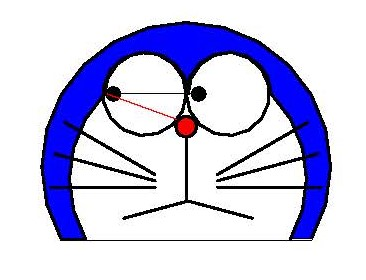
\includegraphics[scale=.3]{doraemon1.jpg}} 
            %* "\titlerule*[width]{text}"命令不填充一条水平直线,而是等距离填充指定内容(可以是图片),必选参数为重复填充内容,可选参数表示等距离填充的盒子宽度,以此来控制填充次数:宽度如果大于图片宽度,宽度越大,填充次数越少(最少填充一次,居中填充);宽度如果小于图片宽度,则也只会填充一次,在右侧填充;如果设置为0pt,则不会显示出填充内容,但是保留其竖直距离,类似于"\vspace{l}"命令和"\rule[lift]{width}{thickness}"命令的“支柱”功能
    \titlerule 
            %* "\titlerule"命令填充一条水平直线,线条高度为默认值0.4pt
    \titleline[c]{\textbackslash titleline没有line}
            %* "\titleline[align]{horizontal material}"命令不填充一条水平直线,而是在水平方向上填充指定内容,可以选择靠左(l)、居中(c)或者靠右(r)填充,默认为靠左填充,填充内容如果超过一行,打印时不会换行,而是超出文本区域继续打印
    \titlerule
    \titlerule*{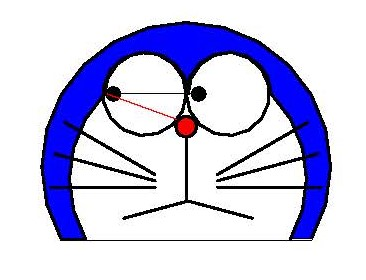
\includegraphics[scale=.3]{doraemon1.jpg}}
            %* "\titlerule*{text}"命令以填充内容的自然宽度进行填充
    \titlerule[.8pt]
            %* 在"\titleformat*{command}{format}"命令或者"\titleformat{command}[shape]{format}{label}{sep}{before-code}[after-code]"命令的{format}参数中也可以使用"\titleline[align]{horizontal material}"命令和"\titlerule*[width]{text}"命令,可以在指定一级章节的上方填充直线或者填充内容,但是无法在其下方进行相同操作
            %todo 是否可以通过某种方式在指定一级章节的下方填充直线或者填充内容,待研究
        \subsubsection{这是一个小节}
            \subsubsubsection{这是一个新定义的小小节}
                这不是段一级,而是新定义的小小节一级。

\section*{不编号的一章}
            %* 该命令设置的章节名称在正文中会打印出来,但是不会编号,在目录中不会打印出来
            \addcontentsline{toc}{section}{不编号的一章}
            %* 该命令设置的章节名称会在目录中打印出来,但是不会编号,在正文中不会打印出来,点击目录中对应的章节名称,索引到该命令在正文中对应的位置,可以发现,该命令类似于一个普通的"\section{}"命令,但是并不会在正文中打印其章节名称
            %! 经检验,上述这一条命令也可以加在除了正文之外的的其他位置,包括导言区,以及"\end{document}"命令之后,编译都不会报错。如果加在导言区,则在目录中会打印在开头,如果加在"\end{document}"之后,则在目录中不会打印出来
            %* 因此,"\section*{title}"命令和"\addcontentsline{file}{secunit}{entry}"命令其实是可以各自独立使用的,但是后者单独使用是没有实际意义的,因为在正文中无法打印出其设置的章节名称。后者实际上只能搭配前者使用,一般将其放置在前者所在的位置之后,这样,在目录中打印出来的章节名称实际上不是前者设置的,而是后者设置的,点击该章节名称实际上也只是索引到后者所在位置,而正文中打印出来的章节名称,则是前者设置的,而不是后者设置的
            %* 结合"\section[short]{title}"命令中可选参数的效果,"\addcontentsline{file}{secunit}{entry}"其实就是将"\section[short]{title}"的可选参数分离出来单独作为一条命令的结果,与之对应的,"\section*{title}"命令就不再含有可选参数,当然,从另一个角度看,"\section*{title}"命令不会在目录中打印章节名,当然没有可选参数存在的必要
 
% 通过重定义"\refname"命令来修改参考文献的标题
            \renewcommand{\tocbibname}{这是参考文献} 
            % 如果是book类文档,把"\refname"改成"\bibname"
            % 如果加载tocbibind宏包,则修改参考文献标题应该重定义"\tocbibname"命令
            %* 在ctexart文档类型下,参考文献标题默认显示“参考文献”,如果加载tocbibind宏包,依然显示“参考文献”,如果加载natbib宏包,则显示“Bibliography”,如果同时加载natbib宏包和tocbibind宏包,依然显示"Bibliography",可见,tocbibind宏包并不改变参考文献的默认标题,而natbib会将参考文献的标题从默认的“参考文献”修改为"Bibliography",但是只要加载了tocbibind宏包,修改参考文献的标题就要通过重定义"\tocbibname"来完成

% 显示所有参考文献
            \begin{thebibliography}{99} % “99”表示以最多两位数来编号参考文献,用于对齐
                \addtolength{\itemsep}{-2ex} % 将参考文献中条目之间的距离减少2ex,注意单个条目内部的行距不会发生变化
                \bibitem{author1.year1}{Au1. ArtName1[J]. JN1. Y:1--2} % 书中在参考文献的形式两边没有加大括号,加与不加,编译的结果相同
                \bibitem{author2.year2}Au2. ArtName2[J]. JN2. Y:1--2
            \end{thebibliography}
            %* 以上都是\LaTeX的原生命令,即使不加载natbib宏包也能编译成功,natbib宏包仅仅是修改了索引的上标形式

% 显示所有尾注
            \theendnotes

\end{document}

